\documentclass[a4paper,12pt]{report}

\usepackage[latin1]{inputenc}
\usepackage{graphicx}

\setlength {\textheight}{247mm}
\setlength {\textwidth}{168mm}
\setlength {\oddsidemargin}{0cm}
\setlength {\evensidemargin}{0cm}
\setlength {\headsep}{0cm}
\setlength {\headheight}{0cm}
\setlength {\topmargin}{0cm}
\setlength {\leftmargin}{0cm}
\setlength {\unitlength}{1cm}
\setlength {\parindent}{0cm}

\title{Implementation of a dynamic invocation interface for AdaBroker}
\author{S\'ebastien Ponce}
\date{\today}

\begin{document}

\maketitle

\begin {abstract}
\paragraph{}The problem you have each time you try to write a documentation is the following : 
how to make it interesting for non specialists without
boring the specialists ? To solve it, we choose to use the same structure as John Barnes did in his ``Programming in ADA 95''.
\paragraph{}So the first part is dedicated to non specialists who need a general presentation of the CORBA concepts. It first
presents what CORBA is (Common Object Request Broker Architecture), then what AdaBroker is (a free, GPL released Ada ORB).
 At last, it describes
the two invocation mechanisms provided in CORBA : the static one and the dynamic one.
\paragraph{}The second part is more specialized and describes in details the implementation of the
Dynamic Invocation Interface in the AdaBroker product. You can find there explanations on all the types
used in the DII (Any, TypeCode, NamedValue, NVList) as well as explanations on the way to build a request and to call the ORB on it.
\end{abstract}

\tableofcontents

%%%%%%%%%%%%%%%%%%%%%%%%%%%%
%%%  Make it simple stupid
%%%%%%%%%%%%%%%%%%%%%%%%%%%%%
\part{Keep It Simple Stupid}

\paragraph{}This first part intends to be readable by everyone (maybe everyone knowing Ada for the last two chapters).
 It briefly presents CORBA and the AdaBroker 
product before explaining the way operations are invoked in AdaBroker, both statically and dynamically.
\paragraph{}Reading this part, you should already be able to build applications using CORBA and AdaBroker. If you need more 
technical information or if you are interested in the way AdaBroker is built, please refer to the next part.

%%%%%  Overview of CORBA
%%%%%%%%%%%%%%%%%%%%%%%%%
\chapter{Overview of CORBA}

\paragraph{}You'll find here a general introduction to CORBA as well as an explanation of the way it works globally.
If you already know something on CORBA, just skip this chapter.
\paragraph{}We'll first describe CORBA in general, then give a little example of a CORBA application and at last speak of some of
the more advanced CORBA features.

%%%  OMG
\section{The OMG}
\paragraph{}The {\bf O}bject {\bf M}anagement {\bf G}roup is a consortium created in 1989 
that puts together more than 850 actors of the new economy :
contructors like Sun or IBM, software sellers like Netscape, Inprise or Visigenic, users like Boeing or Alcatel and institutions or
universities like NASA, INRIA, LIFL. The goal of this group is to create standards for the integration of heterogeneous applications
on distributed systems using object oriented technologies. The key concepts are thus reusability, interoperability and portability
of software components.
\paragraph{}The key element of the OMG vision is CORBA : {\bf C}ommon {\bf O}bject {\bf R}equest {\bf B}roker {\bf A}r\-chi\-tec\-ture.
It is an object oriented middleware that provides an execution support hiding the technical levels of a distributed system (operating
system, processor and network). It deals with all the communications between software components building heterogeneous distributed
applications.
\paragraph{}

%%%  Client-server model
\section{Client - Server architecture}
\paragraph{}As can be expected, CORBA is based on a classical client-server architecture where the clients and the servers communicate
through the so called CORBA Bus.
\paragraph{}There is thus two types of applications using CORBA : 
\begin{itemize}
\item servers, or service furnishers that provide some useful objects to be used by all other CORBA users.
\item clients which place sort of remote procedure calls on the objects provided by the different servers.
\end{itemize}
Figure 1.1 on page \pageref{fig:CSModel} shows you a schema of this process.
\begin{figure}
\label{fig:CSModel}
\begin{center}
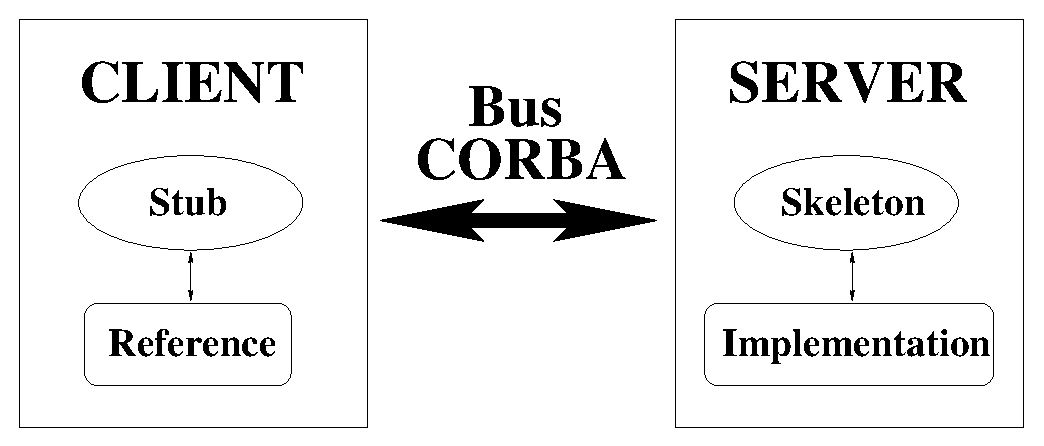
\includegraphics[scale=0.7]{client-server_model.eps}
\caption{Client-Server Model}
\end{center}
\end{figure}

\paragraph{}You can notice on this schema that even inside the client or the server, there are two different levels.
The upper level on each side (Stub for the client and Skeleton for the server) is actually an abstraction level that provides language
independency and distributed facilities. As a matter of fact, CORBA allows the programmers to write code in his prefered language
and without being bored by the distributed aspect. The user, for example uses Object References as if they
were local objects and when he calls methods on them, these are redirected by the stub that performs all the network stuff.
\paragraph{}Let's see a little more in detail how all this work.

%%% Object Definition in IDL
\section{Object definition in IDL}
\paragraph{}IDL stands for {\bf I}nterface {\bf D}efinition {\bf L}anguage since objects are called interfaces in CORBA.
This language provides a way of specifying objects through their interface in order to describe the way they have to be used without
setting limits to the implementation.
\paragraph{}IDL uses a kind of modified C syntax. There is no point to detail this syntax here, just refer to \cite{OMG} if you need further
details. Here is a sample IDL file, defining a calculator service.
\begin{verbatim}
interface calculator {
  long Add (in long a, in long b);
  long Sub (in long a, in long b);
};
\end{verbatim}
\paragraph{}If defines an object {\it calculator} with two methods : Add and Sub taking both two long and returning one.
Now let's see how this file can be used.

%%% Language Mapping
\section{Mapping to a language}
\paragraph{}We said CORBA is language independant and everyone can program in its prefered language. At this moment, we only introduced a
new language : IDL. How does it help ?
\paragraph{}It helps since it gives a common description of the object that will be used in all other languages to generate a language
specific code implementing the object. This operation is called mapping. It is done by compilers that automatically
generate the Stub and Skeleton we saw before in your prefered language. As an example, we show here some results of this
mapping on the calculator object (only the specifications are presented here) :
\begin{itemize}
\item In C++ (using omniOrb)
\begin{verbatim}
class calculator : public virtual omniObject,
                   public virtual CORBA::Object {
public:

  virtual CORBA::Long  Add(CORBA::Long  a, CORBA::Long  b) = 0;
  virtual CORBA::Long  Sub(CORBA::Long  a, CORBA::Long  b) = 0;
  (...)
};
\end{verbatim}
\item In Java (using orbacus)
\begin{verbatim}
public interface calculatorOperations {

    public int Add(int a, int b);
    public int Sub(int a, int b);
}
\end{verbatim}
\item and last but not least : in Ada (using the wonderful AdaBroker)
\begin{verbatim}
package calculator is
   (...)
   function Add (Self : in Ref;
                 a : in CORBA.Long;
                 b : in CORBA.Long)
                 return CORBA.Long;

   function Sub (Self : in Ref;
                 a : in CORBA.Long;
                 b : in CORBA.Long)
                 return CORBA.Long;
   (...)
end calculator;
\end{verbatim}
\end{itemize}
\paragraph{}The CORBA specification defines precisely each of these mappings. For the Ada one, please report to \cite{AdaMapping} 
if you want some details. The writter of both clients and servers can use the mapping they prefer, only dealing with a convenient 
interface written in their own language.

%%% Distributivity
\section{Distributed ?}
\paragraph{}We know at this moment how a client or a server are implemented, in a language independant manner
but what about a distributivity ? Can my client and my server be on different machines, in different places ? The answer is of course : Yes.
This is provided through the definition of the GIOP : the {\bf G}eneral {\bf I}nter{\bf O}RB {\bf P}rotocol.
\paragraph{}This protocol defines the way different machines running a CORBA ORB can communicate to allow clients of one to call servers
on the other. The theory is pretty simple : it defines a way of coding a procedure call (basically an object name, an operation
name and some arguments) and how the result is inserted in a TCP/IP packet or whatever else. It also defines the way the result is
sent back (even when exceptions occurs).
\paragraph{}All these operations of coding, decoding (we call it marshalling and unmarshalling) and dealing with the network are transparent
to the user since they are implemented in the automatically generated Stub and Skeleton. The user can then code its client or server
as if he were only using local objects. Note that this GIOP is also the key of the language independency since the bytes that are sent
over the network are the same for every mapping. They do not depend on the sender language.

%%% Some other features
\section{Some other CORBA features}
CORBA has some more features we didn't spoke of yet. Let's detail some of them.

\subsection{Dynamic Invocation}
\paragraph{}The dynamic invocation is a way of placing a remote procedure call on an object without knowing its specification.
It allows a client
code to invoke a method in a very general manner without using the Stub and Skeleton we spoke of since you're not supposed to
have the IDL specification here. It can seem a bit odd but it is very useful. Most of this document is devoted to the explanation of
this feature and to its implementation in AdaBroker so you know where to find some information.
\subsection{Interface Repository}
\paragraph{}This is actually a CORBA server as many others except it allows you to register some objects (in case you are a server
providing them) and allows then the clients to discover them dynamically. Together with the dynamic invocation, it allows a code to
use some object that didn't even exist when the code was written. This was implemented in AdaBroker by Vincent Niebel.
\subsection{other services}
\paragraph{}The interface repository is not the only service to be defined by the OMG itself. There are a bunch of them and the most
known are cosNaming, cosTime and cosEvent (I let you guess what kind of service they provide).

%%%  Adabroker
%%%%%%%%%%%%%%%%%%%%%
\chapter{Overview of AdaBroker}
\paragraph{}You'll find here a general introduction to AdaBroker, a GPL released Ada ORB for CORBA.

\section{What it is}
\paragraph{}AdaBroker is an Ada ORB for CORBA. It all began with a student project at the ENST 
(Ecole Nationale Sup�rieure des T�l�coms) in Paris, France in Januar 1999. 
The first version (beta 0.8) was released in the summer 99 and already provided most of the existing CORBA features.
It was mostly based on external components since it used the Sun front-end for the parsing of
 Idl and the OmniORB ORB.
\paragraph{}The first major work for the AdaBroker team was to rewrite all the components in Ada in order to provide an independant,
full Ada software. This was achieved in version 1pre1, released in April 2000. The two main components of the AdaBroker software are now :
\begin{itemize}
\item {\bf idlac} as an idl to Ada compiler, full Ada, written by the AdaBroker team
\item {\bf broca} as an ORB, also full Ada, also written by the AdaBroker team
\end{itemize}
\paragraph{}In this 1pre1 version, the features were mostly the same as in the beta 0.8 one :
\begin{itemize}
\item full static invocation mechanism
\item management of exceptions
\item management of forward declarations (to allow recursive definitions)
\item management of multiple inheritance in Idl
\item management of all CORBA types, including sequences, unions and fixed but not values since it didn't exist.
\end{itemize}
Some components were missing to provide a full ORB :
\begin{itemize}
\item Dynamic invocation (both client and server part)
\item management of values
\item interface repository
\item the major services  cosNaming, cosEvent, cosTime...
\end{itemize}
All of these components are currently under developpement and the next release should provide dynamic invocation
(client part), an interface repository, the management of values and some services.
This is the purpose of this document to describe at least the dynamic invocation mechanism on the client side.

\section{How to get it, how to contact us}
You just have to go to http://adabroker.eu.org. You can download the software there and have some information concerning
the mailing lists and current releases. This site is hosted by Ada France.

%%% Static invocation Mechanism
%%%%%%%%%%%%%%%%%%%%%%%%%%%%%%%%%%
\chapter{The static invocation mechanism}
\label{SIM}
\paragraph{}We'll present the static invocation mechanism through the most simple example you can think of : the echoString example.
Just try here to imagine what string we could use to test it (beginning by ``Hello'')... 
\paragraph{}Since this example is a bit simple, it some time does not fit
to describe the general case. We'll always mention it and explain the whole thing.
\paragraph{}Here is the IDL specification of this example :
\begin{verbatim}
interface Echo {
  string echoString (in string Mesg);
};
\end{verbatim}

\paragraph{}The static way to build a client-server application on this IDL interface consists in two steps :
first building the server and then the client.

%%%%%%  Building a Server
\section{Building a server}
\paragraph{}The server itself has two main parts : an implementation, which is the code that effectively 
does the job, here echoing a string, and a skeleton which is an interface between your implementation and the ORB, allowing the ORB to 
call your code.
\paragraph{}Both parts can be generated automatically using an IDL to Ada compiler. Here we use {\it idlac}, provided in the 
AdaBroker package. The skeleton can be fully generated whereas the implementation is just a framework you'll have to fill in.

Note that the implementation is not generated by default, in order not to remove some already filled in files. You have to use the '-i' flag
to generate it.

\subsection{Implementation}
\paragraph{}Let's have a look at the implementation files first. Nothing surprising there. Here is the spec :
\begin{verbatim}
package Echo.Impl is

   type Object is new PortableServer.Servant_Base with null record;

   function echoString (Self : access Object;
                        Mesg : in CORBA.String)
                        return CORBA.String;
end Echo.Impl;
\end{verbatim}
and here is the empty implementation :
\begin{verbatim}
package body Echo.Impl is

   function echoString (Self : access Object;
                        Mesg : in CORBA.String)
                        return CORBA.String is
      Result : CORBA.String;
   begin
      --  Insert implementation of echoString
      return Result;
   end echoString;

end Echo.Impl;
\end{verbatim}
In our case, the implementation is easy to build, we just have to insert ``\texttt{Result := Mesg;}'' where indicated.

\subsection{Skeleton}
\paragraph{}As I already mentionned it, the skeleton files (echo-skel.ads/adb) are fully generated by {\it idlac}. However, it is interesting to have a look at them in order to understand the invocation mechanism.
\paragraph{}Here is the interesting part of echo\_skel.ads :
\begin{verbatim}
   procedure GIOP_Dispatch
     (Obj : PortableServer.Servant;
      Operation : String;
      Request_Id : CORBA.Unsigned_Long;
      Response_Expected : CORBA.Boolean;
      Request_Buffer : access Broca.Buffers.Buffer_Type;
      Reply_Buffer   : access Broca.Buffers.Buffer_Type) is
   begin
      if Operation = "echoString" then
        (...)
         declare
            IDL_Mesg : CORBA.String;
            Return_U : CORBA.String;
         begin
            --  Unmarshall in and inout arguments
            IDL_Mesg := Unmarshall (Request_Buffer);
            begin
               --  Call implementation
               Return_U := Echo.Impl.echoString (Object_Ptr (Obj), IDL_Mesg);
            end;
            (...)
            --  Marshall return value
            Marshall (Reply_Buffer, Return_U);
            return;
         end;
      end if;
      Broca.Exceptions.Raise_Bad_Operation;
   end GIOP_Dispatch;
\end{verbatim}
\paragraph{}This method is actually called by the ORB each time there is a request on the echo object. The only significant arguments 
for us are \texttt{Operation} and the two buffers : \texttt{Request\_Buffer} and \texttt{Reply\_Buffer}. 

What this method does is 
simply looking at the operation name contained by \texttt{Operation}, getting the arguments of this operation from the 
\texttt{Request\_Buffer}, calling the actual implementation of the operation with these arguments
 and puting the result in the \texttt{Reply\_Buffer}.

\paragraph{}There could be some changes if you don't use exactly the same example :
\begin{itemize}
\item{}In case another method were defined on the echo object, you would have another \texttt{if Operation = ... then ... end if;} 
block for this method. Each block is dealing with a single method and the end of the \texttt{GIOP\_Dispatch} method is only reached when none of
the provided methods fits. In this case, an exception is raised. 
\item{}In case you had some out or inout arguments in your method, their return value would have been put
in the \texttt{Reply\_Buffer} with the result.
\item{}In case your implementation potentially raises an exception, this one must have been specified in the IDL specification as in :
\label{StaticExcp}
\begin{verbatim}
interface Echo {
  exception Bad_String { long Bad_Character_Index; };
  string echoString (in string Mesg) raises (Bad_String);
};
\end{verbatim}
The generated code will then take this situation into account and put the exception into the \texttt{Reply\_Buffer}. Here is this generated
code :
\begin{verbatim}
      begin
         --  Call implementation
         Return_� := Echo.Impl.echoString (Object_Ptr (Obj),
                                     IDL_Mesg);
      exception
         when E : Echo.Bad_String =>
            declare
               Members_� : Echo.Bad_String_Members;
            begin
               Echo.Get_Members (E, Members_�);
               (...)
               --  Marshall exception
               Marshall (Reply_Buffer, CORBA.String
                 (Echo.Bad_String_Repository_Id_�));
               Marshall (Reply_Buffer, Members_�);
               return;
            end;
      end;
\end{verbatim}
\end{itemize}

%%%%%%  Building a Client
\section{Building a client}
We are here in the position of the user, that has just discovered the unbelievable power of the echo object and wants to use it remotely
in his application. Once more, there is two main parts in the code we'll need. The first part is the client application and the second one
a kind of proxy called {\it stub} being able to talk with the ORB and make it
execute remotely the method (possibly in an other language, on an other architecture).

\subsection{A proxy to the ORB}

\paragraph{}This ``proxy'' is provided by the echo.ads and echo.adb files. Here is the main code of echo.ads :
\begin{verbatim}
package Echo is
   type Ref is new CORBA.Object.Ref with null record;

   function echoString (Self : in Ref;
                        Mesg : in CORBA.String)
                        return CORBA.String;
   (...)
end Echo;
\end{verbatim}

\paragraph{}We found here the definition of the echo object and the \texttt{echoString} method the client is interested in.
Here is the implementation of the \texttt{echoString} method in echo.adb :
\begin{verbatim}
   function echoString (Self : in Ref;
                        Mesg : in CORBA.String)
                        return CORBA.String is
      Handler_U : Broca.GIOP.Request_Handler;
      Send_Request_Result_U : Broca.GIOP.Send_Request_Result_Type;
      Return_U : CORBA.String;
   begin
      (...)
      loop
         --  Create a buffer and marshall the operation name
         Broca.GIOP.Send_Request_Marshall
            (Handler_U,
             Broca.Object.Object_Ptr (Get (Self)),
             True,
             echoString_Operation);

         --  Marshall in and inout arguments for the operation
         Marshall (Handler_U.Buffer'Access, Mesg);

         --  Send a request to the ORB
         Broca.GIOP.Send_Request_Send (Handler_U, 
                                       Broca.Object.Object_Ptr (Get (Self)),
                                       True,
                                       Send_Request_Result_U);

         --  Unmarshall return value.
         case Send_Request_Result_U is
            when Broca.GIOP.Sr_Reply =>
               Return_U := Unmarshall (Handler_U.Buffer'Access);
               Broca.GIOP.Release (Handler_U);
               return Return_U;
            (...)
         end case;
      end loop;
   end echoString;
\end{verbatim}

\paragraph{}The way it works is really simple : it creates a buffer where it marshalls (understand puts) the operation name and arguments,
then it calls the ORB giving this buffer to it and at last, it gets back the result.

You could find some modifications with other examples :
\begin{itemize}
\item{}If there was another method in echo, we'd have two generated methods, each calling the ORB with its own name and arguments.
\item{}If a method had out or inout arguments, we could get back their value from the same buffer where we got back the result.
\item{}If a method potentially raises an exception, the generated code would take that into account. The last case
(on \texttt{Send\_Request\_Result\_U}) would have another when item looking like this :
\begin{verbatim}
   when Broca.GIOP.Sr_User_Exception =>
      declare
         Exception_Repo_Id_� : constant CORBA.RepositoryId
           := CORBA.RepositoryId (CORBA.String'
              (Unmarshall (Handler_�.Buffer'Access)));
      begin
         if CORBA."=" (Exception_Repo_Id_�,
                       Echo.Bad_String_Repository_Id_�) then
            declare
               Members_� : constant Echo.Bad_String_Members
                 := Unmarshall (Handler_�.Buffer'Access);
            begin
               (...)
               Broca.Exceptions.User_Raise_Exception
                 (Echo.Bad_String'Identity,
                  Members_�);
            end;
         end if;
         (...)
      end;
\end{verbatim}
\end{itemize}

\subsection{A client}
\paragraph{}The client is very simple to write since the invocation of the \texttt{echoString} method looks like as if it were local.
\begin{verbatim}
procedure Client is
   Sent_Msg, Rcvd_Msg, IOR : CORBA.String;
   myecho : Echo.Ref;
begin
  (...)
   --  transforms the Ada string into CORBA.String
   IOR := CORBA.To_CORBA_String (Ada.Command_Line.Argument (1));

   --  gets a reference on the server we want to use
   CORBA.ORB.String_To_Object (IOR, myecho);

   --  actual call to the method, through the ORB
   Sent_Msg := CORBA.To_CORBA_String 
      (Standard.String'("Hello Static World !"));
   Rcvd_Msg := Echo.echoString (myecho, Sent_Msg);
   (...)
end Client;
\end{verbatim}

\paragraph{}Nothing to add here except that you have to give to the client what is called an IOR which is a reference to the server
you intend to use. This could be avoid by using the cosNaming service.

%%%%% What was static
\section{Conclusion : how was it static ?}
\paragraph{}Or what could be dynamic ?

\paragraph{}We saw through this example the absolute necessity for both the client and the server to compile the IDL interface through
an IDL compiler such as {\it idlac}. If you don't have it, you cannot call the ORB on the client side, and you cannot be called on the
server side. This implies that both client and server are very dependant on the IDL compiler (if this one changes, you'll have to change
your code) and on the IDL interface (you have to know all of it). That's what is considered as static in the whole thing.

\paragraph{}On the other hand, we would call dynamic an invocation that won't use the IDL compiler and will allow one client to adapt
to the server, discovering what methods it has and what kind of arguments it needs before calling it. That's exactly what the DII
(Dynamic Invocation Interface) proposes.

\paragraph{}Apart from these considerations on static/dynamic calls, did you notice that all the invocations to the ORB, in the client
part, were blocking ? That will be another feature of the dynamic invocation : the possibility to place asynchronous calls.

%%%% DII
%%%%%%%%%%%%%%%%
\chapter{The dynamic invocation mechanism}
\label{cha:DIM}
\paragraph{}In the previous chapter, we saw all the static invocation mechanism and its limitations.
We present here the solution to these limitations : the dynamic invocation mechanism.

\paragraph{}The Dynamic Invocation Mechanism is supported on the client side by the Dynamic Invocation Interface. The idea here is to write a
kind of generic proxy that would be used for every existing object, instead of having one proxy per object. This proxy would be
able to marshall the operation name and arguments exactly in the same way as a dedicated proxy, so that the ORB and the server
will never know if the invocation was dynamic or not.

\paragraph{}In order to write such a generic proxy, you'll need some way of passing generic arguments to it. It means you need 
a self-describing type that is able to encapsulate any given value. This type is called \texttt{Any}; it is associated with the
\texttt{TypeCode} type used to describe any value type.

\paragraph{}Giving these generic types and a generic proxy, all works fine. Lets look further in all this, using the same example 
we used in chapter \ref{SIM}, page \pageref{SIM}.

%%% Dynamic Types
\section{Dynamic types}
\paragraph{}There's a bunch of new types using in the dynamic invocation. There are pretty complex but easy to use.
Here is a kind of gallery of them with the informations you'll need to use them.
\paragraph{}Just a last thing : all the methods provided for dynamic invocation and dealing with user defined types are generated by
idlac in the helper package corresponding to the package where the type was defined. If you don't want to use these package (because
you don't have the IDL specification or the compiler), you can create Any using the DynAny type but that's not implemented in
AdaBroker nor explained here.

\subsection{TypeCode}
\paragraph{}This type encapsulates a type definition. He's pretty opaque for the user but you don't need to know what's inside.
The only thing to know is that every given type has its corresponding TypeCode constant, which name is TC\_{\it name\_of\_type}.

\subsection{Any}
\paragraph{}This type encapsulates any value that could be used in CORBA. This is a self-describing type. It actually contains a
TypeCode (you cen get it by using the {\it Get\_Type} function and a value of this type.
\paragraph{}It is the base of all the dynamic invocation since the generic proxy should be able to send every kind of value to
the ORB. The value it takes are thus Anys. Last thing : you can create Anys by using {\it To\_Any} methods (that are provided for every
type) and get their value back by using {\it From\_Any} methods (also provides for every type).

\subsection{NamedValue}
\paragraph{}This type encapsulated the description of an argument to be passed to a method. Its definition is public :
\begin{verbatim}
   type NamedValue is record
      Name :      CORBA.Identifier;
      Argument :  CORBA.Any;
      Arg_Modes : CORBA.Flags;
   end record;
\end{verbatim}
\paragraph{}It contains the name of the parameter, its value and its mode (ARG\_IN, ARG\_OUT or ARG\_INOUT).

\subsection{NVList}
\paragraph{}This is only a list of NamedValues. It has some useful methods :
\begin{verbatim}
   procedure Add_Item
     (Self : Ref;
      Item : in CORBA.NamedValue);
   function Get_Count (Self : Ref) return CORBA.Long;
\end{verbatim}
And an NVList can be created (empty) using a method in package {\it CORBA.ORB} :
\begin{verbatim}
   procedure Create_List
     (Count    : in     CORBA.Long;  --  useless, put 0 there
      New_List :    out CORBA.NVList.Ref);
\end{verbatim}

%%% The generic Proxy
\section{The generic proxy}
\paragraph{}We'll describe here the way the dedicated proxies were replaced by a generic one. This is done by using the package request
and especially its {\it Invoke} method.

\subsection{The {\it Request} package}
The generic proxy is provided through the {\it CORBA.Request} package and its invoke method. This package allows the user to describe
precisely the invocation he intends to do while building a request and to send it to the ORB then. The main methods of this package
(in the case of a blocking operation) are :
\begin{verbatim}
package CORBA.Request is

   type Object is private;

   procedure Add_Arg
     (Self : in out Object;
      Arg  : in     NamedValue);

   procedure Invoke
     (Self         : in out Object;
      Invoke_Flags : in     Flags  := 0);

end CORBA.Request;
\end{verbatim}

\paragraph{}Added to that, there is a kind of constructor for requests provided in the {\it CORBA.Object} package :
\begin{verbatim}
   procedure Create_Request
     (Self      : in     Ref;
      Ctx       : in     CORBA.Context.Ref;
      Operation : in     Identifier;
      Arg_List  : in     CORBA.NVList.Ref;
      Result    : in out NamedValue;
      Request   :    out CORBA.Request.Object;
      Req_Flags : in     Flags);
\end{verbatim}

\paragraph{}The {\it Create\_Request} methods gets all the informations that were needed to generate the dedicated proxy in the case
of a static in vocation. We find there :
\begin{itemize}
\item{\it Self} which is a reference to the object to be called. In our case, an {\it Object.Ref} replacing the former {\it echo.Ref}.
\item{\it Ctx} which is the context of the invocation. We don't need to understand that at this point. Note that it was also taken into
account in the static invocation.
\item{\it Operation} which is the name of the operation to be invoked : ``{\it echoString}'' in our case
\item{\it Arg\_List} : This is the key argument : it contains all the arguments to be passed to the invoked method, 
as a list of Any. See chapter \ref{NV-NVList} on page \pageref{NV-NVList} for further information on the type of this argument.
All what you need to know for the moment is how to create it and this will be explained soon.
\item{\it Result} which is an any where the result of the operation may be stored (if it exists). Note that it is an inout argument since the
type of the result must already be set when {\it Create\_Request} is called and this type is part of the Any.
\item{\it Request} which is the built request Object.
\item{\it Req\_Flags} are flags to specify some memory management policy. Forget it here.
\end{itemize}
\paragraph{}After a call to {\it Create\_Request}, the resulting request describes exactly the invocation that we intend to do.
You can add some more arguments in you want, using {\it Ard\_Arg} and when you're ready, you just have to call invoke on your request.

\subsection{Getting back the results}
\paragraph{}when {\it Invoke} is called, the result (if it is a function) and the out args are directly put into the NamedValues that
were put into the request. Thus, there is no method to get it back from the Request object. Here is an example since a short example
is better than a long speech :
\begin{verbatim}
declare
   Args : NVList := (...);
   Result : NamedValue := (...);
   Request : CORBA.Request.Object;
begin
   Create_Request (... , Args, Result, Request, ...);
   Invoke (0, Request)
   --  here you can use Result and Args
   --  the new values are there
end;
\end{verbatim}

\subsection{The invocation}
\paragraph{}Since we are discussing the differences between static and dynamic invocation, let's look a bit further at what is done
in the {\it Invoke} method. Here is part of its code :
\begin{verbatim}
   procedure Invoke
     (Self         : in out Object;
      Invoke_Flags : in     Flags  := 0) is
      Handler : Broca.GIOP.Request_Handler;
      Send_Request_Result : Broca.GIOP.Send_Request_Result_Type;
   begin
      loop
         --  create a buffer and marshall the operation name
         Broca.GIOP.Send_Request_Marshall 
           (Handler,
            Broca.Object.Object_Ptr 
               (CORBA.AbstractBase.Get (Self.Target)),
            True,
            Self.Operation);

         --  Marshall in and inout arguments.
         CORBA.NVList.Marshall (Handler.Buffer'Access,
                                Self.Args_List);

         --  send the request
         Broca.GIOP.Send_Request_Send
           (Handler,
            Broca.Object.Object_Ptr 
               (CORBA.AbstractBase.Get (Self.Target)),
            True,
            Send_Request_Result);

         case Send_Request_Result is
            when Broca.GIOP.Sr_Reply =>
               --  Unmarshall out args
               CORBA.NVList.Unmarshall (Handler.Buffer'Access,
                                        Self.Args_List);

               --  Unmarshall return value
               Self.Result := Broca.CDR.Unmarshall
                 (Handler.Buffer'Access,
                  Self.Result.Name,
                  CORBA.Get_Type (Self.Result.Argument),
                  Self.Result.Arg_Modes);
               Broca.GIOP.Release (Handler);
               return;
         (...)
         end case;
      end loop;
   end Invoke;
\end{verbatim}
Looks pretty like the former dedicated proxy, hum ? The only difference is the way the arguments and results are marshalled and 
unmarshalled but be sure the effects in the buffer are the same.

%%% The new client code
\section{The new client code}
\paragraph{}As you can imagine, the client code in the dynamic invocation mechanism is a bit longer than in the static case, 
since you do part of the job of the former proxy by building a list of arguments.
\paragraph{}Here is what it looks like :
\begin{verbatim}
procedure DynClient is
   Sent_Msg : CORBA.String := To_CORBA_String ("Hello Dynamic World");
   Operation_Name : CORBA.Identifier := To_CORBA_String ("echoString");
   Arg_Name : CORBA.Identifier := To_CORBA_String ("Mesg");
   IOR : CORBA.String;
   myecho : CORBA.Object.Ref;
   Request : CORBA.Request.Object;
   Ctx : CORBA.Context.Ref;
   Argument : CORBA.Any;
   Arg_List : CORBA.NVList.Ref;
   Result : CORBA.NamedValue;
   Result_Name : CORBA.String := To_CORBA_String ("Result");
   Recv_Msg : CORBA.String;
begin
   --  transforms the Ada string into CORBA.String
   IOR := CORBA.To_CORBA_String (Ada.Command_Line.Argument (1));

   --  gets a reference on the server we want to use
   CORBA.ORB.String_To_Object (IOR, myecho);

   --  creating the argument list
   CORBA.ORB.Create_List (0, Arg_List);
   Argument := CORBA.To_Any (Sent_Msg);
   CORBA.NVList.Add_Item (Arg_List,
                          Arg_Name,
                          Argument,
                          CORBA.ARG_IN);

   --  setting the result type
   Result := (Name => Identifier (Result_Name),
              Argument => Get_Empty_Any (CORBA.TC_String),
              Arg_Modes => 0);

   --  creating a request
   CORBA.Object.Create_Request (myecho,
                                Ctx,
                                Operation_Name,
                                Arg_List,
                                Result,
                                Request,
                                0);

   --  sending message
   CORBA.Request.Invoke (Request, 0);

   --  getting the answer
   Recv_Msg := From_Any (Result.Argument);

   --  printing result
   Put_Line ("I said : " & CORBA.To_Standard_String (Sent_Msg));
   Put_Line ("The object answered : " & CORBA.To_Standard_String (Recv_Msg));

end DynClient;
\end{verbatim}
\paragraph{}You can notice here the way of handling {\it Any} types or argument lists.
For a more complete description of this, please see part \ref{BigPicture} on page \pageref{BigPicture}.

%%% Special features
\section{Special features}
\paragraph{}The example given does not fit to describe all features of the dynamic invocation. Here is a description of those
we didn't spoke of.

\subsection{Exceptions}
\paragraph{}Exceptions can be raised by a method, be it invoked dynamically or not. As we've already seen it, this is specified in IDL
and thus should be given to the {\it Request} object while creating it. This is possible by using a second {\it Create\_Request} method
whose specification is :
\begin{verbatim}
   procedure Create_Request
     (Self      : in     Ref;
      Ctx       : in     CORBA.Context.Ref;
      Operation : in     Identifier;
      Arg_List  : in     CORBA.NVList.Ref;
      Result    : in out NamedValue;
      Exc_List  : in     ExceptionList.Ref;
      Ctxt_List : in     ContextList.Ref;
      Request   :    out CORBA.Request.Object;
      Req_Flags : in     Flags);
\end{verbatim}
\paragraph{}There is two more parameters there : an {\it ExceptionList} and a {\it ContextList}. We won't speak here of the {\it ContextList}
package since it is not implemented. You just have to put {\it Contextlist.Nil\_Ref} for this parameter. The {\it ExceptionList}
package however allows you to pass a list of potentially raised exception.
\paragraph{}This package is mapped from the {\it NVList} package, the most useful functions are :
\begin{verbatim}
   function Get_Count (Self : in Ref)
                       return CORBA.Unsigned_Long;

   procedure Add (Self : in Ref;
                  Exc : in CORBA.TypeCode.Object);

   function Item (Self : in Ref;
                  Index : in CORBA.Unsigned_Long)
                  return CORBA.TypeCode.Object;

   procedure Remove (Self : in Ref;
                     Index : in CORBA.Unsigned_Long);
\end{verbatim}
All very clear. You can notice that you have to use here the TypeCode associated with each exception.
\paragraph{}In case an exception is raised in the server, it won't be raised as is in the client since this one doesn't know the exception
in a dynamic context. The exception raised will then be a {\it UnknownUserException} with a member ({\it IDL\_Exception})
containing an Any where the value of the member of the exception raised in the server is to be found.
\paragraph{}Here is a sample of the code that could be written :
\begin{verbatim}
    declare
       Member : UnknownUserException_Members;
       Actual_Member : Bad_String_Members;
    begin
    --  dynamic all here       
    exception
       when E : UnknownUserException =>
          Get_Members (E, Member);
          Actual_Member :=
            Echo.Helper.From_Any (Member.IDL_Exception);
          --  here you can use Actual_Member.Bad_Character_Index
    end;
\end{verbatim}

\subsection{Asynchronous invocation}
\paragraph{}One of the major add-on of the dynamic invocation is the ability to place a non-blocking calls. This is provided once more 
by the {\it Request} package through the following functions :
\begin{itemize}
\item{\bf Send} : it invokes the operation like {\it Invoke} but gives you the control right back without waiting the operation to
finish.
\item{\bf Get\_Response} This is the pending of the {\it Send} method. It allows you to get the result of an invocation made with 
{\it Send}. This method is blocking if the result is not yet ready.
\item{\bf Poll\_Response} This allows you to know if a given result is ready or not. This way, you are able 
call {\it Get\_Response} only when you know you won't wait.
\end{itemize}
The only problem here is that none of these functions are provided in AdaBroker at this time...

%%% Conclusion
\section{Conclusion}
\paragraph{}We solved here two out of the three problems the static invocation raised :
\begin{itemize}
\item{}You don't need an Idl to Ada compiler anymore (except without DynAny, it's still better to have one).
\item{}You can avoid blocking invocations.
\end{itemize}
\paragraph{}The last point remains : you have to know the Idl. Right, but if you could imagine a way to discover it, you could use it.
So half of the work is done. For the other half, that's exactly the concern of the Interface Repository.

%%%%%%%%%%%%%%%%%%%%%%%
%%% The Big Picture
%%%%%%%%%%%%%%%%%%%%%%%
\part{The Big Picture}
\label{BigPicture}

\paragraph{}Here we'll present in detail the implementation of the DII in AdaBroker. Each type and package is described and 
explained precisely. 
\paragraph{}We'll begin with a description of the generic types {\it TypeCode} and {\it Any}. Then comes the description of the 
way arguments are stored (type {\it NamedValue} and package {\it NVList}). Then we'll speak of the way {\it Request} is implemented
and the marshalling and unmarshalling is done. At last, we'll deal with some packages that are not essential but useful :
{\it CORBA.ExceptionList}, {\it CORBA.Context} and  {\it CORBA.ContextList}.

%%% typecodes
%%%%%%%%%%%%%%
\chapter{Typecodes}

\paragraph{}{\it TypeCode} is the type used for describing any given value type. It is defined as a subpackage of package {\it CORBA}.
\paragraph{}We'll first describe here the way {\it TypeCode} is implemented in AdaBroker before talking about the methods provided.

%%% Typecodes spec
\section{The Ada specification}
\paragraph{}The following specification is inside the {\it CORBA} package :

\begin{verbatim}
   type TCKind is
      (Tk_Null, Tk_Void, Tk_Short, Tk_Long, Tk_Ushort, Tk_Ulong, Tk_Float,
       Tk_Double, Tk_Boolean, Tk_Char, Tk_Octet, Tk_Any, Tk_TypeCode, 
       Tk_Principal, Tk_Objref, Tk_Struct, Tk_Union, Tk_Enum, Tk_String, 
       Tk_Sequence, Tk_Array, Tk_Alias, Tk_Except, Tk_Longlong, Tk_Ulonglong,
       Tk_Longdouble, Tk_Widechar, Tk_Wstring, Tk_Fixed, Tk_Value, 
       Tk_Valuebox, Tk_Native, Tk_Abstract_Interface);

   type ValueModifier is new Short;
   VTM_NONE : constant ValueModifier;
   VTM_CUSTOM : constant ValueModifier;
   VTM_ABSTRACT : constant ValueModifier;
   VTM_TRUNCATABLE : constant ValueModifier;

   type Visibility is new Short;
   PRIVATE_MEMBER : constant Visibility;
   PUBLIC_MEMBER : constant Visibility;

   package TypeCode is

      type Object is private;
      (...)
      
      function "=" (Left, Right : in Object) return Boolean;
      function Equal (Left, Right : in Object) return Boolean renames "=";
      function Equivalent (Left, Right : in Object)
                           return Boolean;

      function Get_Compact_TypeCode (Self : in Object)
                                     return Object;

      function Kind (Self : in Object) return TCKind;

      function Id (Self : in Object)
                   return CORBA.RepositoryId;

      function Name (Self : in Object)
                     return CORBA.Identifier;

      function Member_Count (Self : in Object)
                             return CORBA.Unsigned_Long;

      function Member_Name (Self  : in Object;
                            Index : in CORBA.Unsigned_Long)
                            return CORBA.Identifier;

      function Member_Type
        (Self  : in Object;
         Index : in CORBA.Unsigned_Long) return Object;

      function Member_Label
          (Self  : in Object;
           Index : in CORBA.Unsigned_Long) return CORBA.Any;

      function Discriminator_Type (Self : in Object)
                                   return Object;

      function Default_Index (Self : in Object)
                              return CORBA.Long;

      function Length (Self : in Object)
                       return CORBA.Unsigned_Long;

      function Content_Type (Self : in Object) return Object;

      function Fixed_Digits (Self : in Object)
                             return CORBA.Unsigned_Short;

      function Fixed_Scale (Self : in Object)
                            return CORBA.Short;

      function Member_Visibility
        (Self  : in Object;
         Index : in CORBA.Unsigned_Long) return Visibility;

      function Type_Modifier (Self : in Object)
                              return CORBA.ValueModifier;

      function Concrete_Base_Type (Self : in Object)
                                   return Object;
   end TypeCode;

   --  pre-defined TypeCode "constants"
   function TC_Null               return TypeCode.Object;
   function TC_Void               return TypeCode.Object;
   function TC_Short              return TypeCode.Object;
   function TC_Long               return TypeCode.Object;
   function TC_Long_Long          return TypeCode.Object;
   function TC_Unsigned_Short     return TypeCode.Object;
   function TC_Unsigned_Long      return TypeCode.Object;
   function TC_Unsigned_Long_Long return TypeCode.Object;
   function TC_Float              return TypeCode.Object;
   function TC_Double             return TypeCode.Object;
   function TC_Long_Double        return TypeCode.Object;
   function TC_Boolean            return TypeCode.Object;
   function TC_Char               return TypeCode.Object;
   function TC_Wchar              return TypeCode.Object;
   function TC_Octet              return TypeCode.Object;
   function TC_Any                return TypeCode.Object;
   function TC_TypeCode           return TypeCode.Object;
   function TC_String             return TypeCode.Object;
   function TC_Wide_String        return TypeCode.Object;
\end{verbatim}

%%% Implementation
\section{TypeCode Implementation}
\paragraph{}{\it TypeCode} isn't a complicated type. Here is its private definition in the AdaBroker code :
\begin{verbatim}
      type Object is
         record
            Kind : CORBA.TCKind := Tk_Void;
            Parameters : Cell_Ptr := null;
         end record;
\end{verbatim}
\paragraph{}where {\it Cell\_Ptr} is a simple list of Any declared as follow :
\begin{verbatim}
      type Cell;
      type Cell_Ptr is access all Cell;
      type Cell is record
         Parameter : CORBA.Any;
         Next : Cell_Ptr;
      end record;
\end{verbatim}

\paragraph{}If it is your first time in this matter, remember that {\it Any} is a self-describing encapsulation of a value 
(it actually contains a {\it TypeCode} to describe the type of the value).
The way it works is that {\it TC\_Kind} gives the general kind of the encapsulated type (such as struct, union, long, ...)
and the list of {\it Any} is precises it a bit the type when it is not a simple
one. For example is {\it Kind} is {\it TC\_Struct}, {\it Parameters} will contain a description of each field type;
if {\it Kind} is {\it TC\_Array}, it will contain its length and so on for other types...

\paragraph{}Here is a table of the signification of the {\it Parameter} list for each Kind of {\it TypeCode}. Each Parameter is
written in the form {\it type (name)} where {\it type} describes the parameter type and {\it name} the parameter meaning. 
Some parameters are repeated in sequence. It is written in the form {\it \{parameters\}}.
\begin{center}
\begin{small}
\begin{tabular}{|l|p{10cm}|}
\hline
{\it TC\_Kind} &
{\it Any}s in {\it Parameter} \\ \hline \hline
 {\bf Tk\_Null} &
-none-\\ \hline
{\bf Tk\_Void} &
-none-\\  \hline
{\bf Tk\_Short} &
-none-\\  \hline
{\bf Tk\_Long} &
-none-\\  \hline
{\bf Tk\_Ushort} &
-none-\\  \hline
{\bf Tk\_Ulong} &
-none-\\  \hline
{\bf Tk\_Float,} &
-none-\\  \hline
{\bf Tk\_Double} &
-none-\\  \hline
{\bf Tk\_Boolean} &
-none-\\  \hline
{\bf Tk\_Char} &
-none-\\  \hline
{\bf Tk\_Octet} &
-none-\\  \hline
{\bf Tk\_Any} &
-none-\\  \hline
{\bf Tk\_TypeCode} &
-none-\\  \hline
{\bf Tk\_Principal} &
-none-\\  \hline
{\bf Tk\_Objref} &
string (Name),

string (RepositoryId)\\  \hline
{\bf Tk\_Struct} &
string (Name),

string (RepositoryId),

\{TypeCode (member type),

string (member name)\}\\  \hline
{\bf Tk\_Union} &
string (Name),

string (RepositoryId),

TypeCode (discriminator type),

\{{\it discriminator type}\footnotemark[1]
(label value),

TypeCode (member type),

string (member name)\}\\  \hline
{\bf Tk\_Enum} &
string (Name),

string (RepositoryId),

\{string (member name)\}\\  \hline
{\bf Tk\_String} &
ulong (max length\footnotemark[2])\\  \hline
{\bf Tk\_Sequence} &
ulong (max length\footnotemark[3]),

TypeCode (element type)\\  \hline
{\bf Tk\_Array} &
ulong (length),

TypeCode (element type)\\  \hline
{\bf Tk\_Alias} &
string (Name),

string (RepositoryId),

TypeCode (aliased type)\\  \hline
\end{tabular}
\end{small}
\end{center}
\footnotetext[1]{for unbounded strings, this value is 0.}
\footnotetext[2]{for unbounded sequences, this value is 0.}
\footnotetext[3]{The type of union label values is determined by the third parameter, {\it discriminator type}}
\begin{center}
\begin{small}
\begin{tabular}{|l|p{10cm}|}
\hline
{\it TC\_Kind} &
{\it Any}s in {\it Parameter} \\ \hline \hline
{\bf Tk\_Except} &
string (Name),

string (RepositoryId),

\{TypeCode (member type),

string (member name)\}\\  \hline
{\bf Tk\_Longlong} &
-none-\\  \hline
{\bf Tk\_Ulonglong} &
-none-\\  \hline
{\bf Tk\_Longdouble} &
-none-\\  \hline
{\bf Tk\_Widechar} &
-none-\\  \hline
{\bf Tk\_Wstring} &
ulong (max length\footnotemark[4]) \\  \hline
{\bf Tk\_Fixed} &
ushort (digits),

short (scale)
\\  \hline
{\bf Tk\_Value} &
string (Name, may be empty),

string (RepositoryId),

short (ValueModifier),

TypeCode (Concrete Base)\footnotemark[5],

\{short (Visibility),

TypeCode (member type),

string (member name)\}\\  \hline
{\bf Tk\_Valuebox} &
string (Name),

string (RepositoryId),

TypeCode (type)\\  \hline
{\bf Tk\_Native} &
string (Name),

string (RepositoryId)\\  \hline
{\bf Tk\_Abstract\_Interface} &
string (Name),

string (RepositoryId)\\  \hline
\end{tabular}
\end{small}
\end{center}
\footnotetext[4]{for unbounded wide strings, this value is 0.}
\footnotetext[5]{should be {\it Tk\_Null} if there is no concrete base}

\paragraph{}This way, we can describe any type that a user could define in the IDL language. Let's see now how the {\it TypeCode} type can be used.

%%% methods provided for typecodes
\section{Methods on TypeCodes}

There is three kinds of method defined in the specification of the TypeCode type. The ones for working on it ({\it Equal},
{\it Equivalent} and {\it Get\_Compact\_TypeCode}), the others to be able to read the parameter list (all the rest in the package itself)
and the last to build {\it Typecode} objects. Apart from these, we added some new ones to help writing, building and marshalling TypeCodes.

\subsection{working on TypeCodes}

Here is a description of each method :
\begin{itemize}
\item{\bf Equal} This is a ``simple'' comparison method on TypeCode. I put quotes on simple because it is not so obvious to see if 
TypeCodes are equal or not. The OMG normalisation says : \textsl {``The equal operation returns TRUE if and only if for
 the target TypeCode 
and the TypeCode passed through the parameter Tc (forget the names, they change in Ada), the set of legal operations is the same and 
invoking any operation from that set on the two TypeCodes return identical result''}.

As a result, the comparison operator checks if the kind of each TypeCode are identical and then compares recursively all the parameters.
\item{\bf Equivalent} ``\textsl{The equivalent operation is used by the ORB when determining type equivalence for values stored in an
IDL any}'' says the norm. The way it should work is pretty precise, here is the semantics given by the norm :
\begin{itemize}
{\it
\item If the result of the kind operation on either TypeCode is tk\_alias, recursively
replace the TypeCode with the result of calling content\_type, until the kind is no longer tk\_alias.
\item If results of the kind operation on each typecode differ, equivalent returns false.
\item If the id operation is valid for the TypeCode kind, equivalent returns TRUE if
the results of id for both TypeCodes are non-empty strings and both strings are equal. 
If both ids are non-empty but are not equal, then equivalent returns FALSE. If either
 or both id is an empty string, or the TypeCode kind does not support the id operation,
 equivalent will perform a structural comparison of the TypeCodes by comparing the 
results of the other TypeCode operations in the following bullet items (ignoring aliases
 as described in the first bullet.). The structural comparison only calls operations
 that are valid for the given TypeCode kind. If any of these operations do not return
 equal results, then equivalent returns FALSE. If all comparisons are equal, equivalent returns true.
\item The results of the name and member\_name operations are ignored and not compared.
\item The results of the member\_count, default\_index, length, digits, and scale
operations are compared.
\item  The results of the member\_label operation for each member index of a union
TypeCode are compared for equality. Note that this means that unions whose members
 are not defined in the same order are not considered structurally equivalent.
\item The results of the discriminator\_type and member\_type operation for each
member index, and the result of the content\_type operation are compared by recursively calling equivalent.
}
\end{itemize}
As you maybe noticed, there is a lack of specification concerning values. So the implementation adds two new items to the preceding list :
\begin{itemize}
\item The results of the member\_visibility and type\_modifier operation are compared.
\item The results of the concrete\_base\_type are compared by recursively calling equivalent.
\end{itemize}
\item{\bf Get\_Compact\_TypeCode} Not implemented in AdaBroker.
\end{itemize}

\subsection{dealing with the parameter list}

\paragraph{}As you can imagine, each method of this kind is returning the value contained
 by the corresponding parameter of a given TypeCode. However,
every operation cannot be called on every TypeCode. If you call an operation that is not allowed for a given TypeCode, a {\it BadKind}
exception will be raised. Apart from that, some methods can raise a {\it Bounds} exception. This is only the case for methods returning
a parameter from a parameter sequence, if the sequence is not long enough compared to the index given.

Here are the Ada specification for these two exceptions : 
\begin{verbatim}
      Bounds : exception;
      type Bounds_Members is new CORBA.IDL_Exception_Members
         with null record;

      BadKind : exception;
      type BadKind_Members is new CORBA.IDL_Exception_Members
         with null record;
\end{verbatim}

\paragraph{}To help you knowing which method can be called on which TypeCode and vice versa, here are two tables with the correspondances.

\paragraph{}First which TypeCode is accepted by each method :
\begin{center}
\begin{small}
\begin{tabular}{p{7,5cm}p{8cm}}
\begin{tabular}{|p{2,8cm}|p{3,8cm}|} \hline
Method & Kind accepted \\ \hline \hline
Kind & every TypeCode \\ \hline
Id & Tk\_Objref  

Tk\_Struct  

Tk\_Union  

Tk\_Enum  

Tk\_Alias  

Tk\_Value  

Tk\_Valuebox  

Tk\_Native  

Tk\_Abstract\_Interface  

Tk\_Except \\ \hline
Name &  Tk\_Objref  

Tk\_Struct  

Tk\_Union  

Tk\_Enum  

Tk\_Alias  

Tk\_Value  

Tk\_Valuebox  

Tk\_Native  

Tk\_Abstract\_Interface  

Tk\_Except \\ \hline
Member\_Count,

Member\_Name & Tk\_Struct  

Tk\_Except  

Tk\_Union  

Tk\_Enum  

Tk\_Value \\ \hline
\end{tabular} &
\begin{tabular}{|p{3,8cm}|p{2,8cm}|} \hline
Method & Kind accepted \\ \hline \hline
Member\_Type & Tk\_Struct  

Tk\_Except  

Tk\_Union  

Tk\_Value \\ \hline
Member\_Label,

Discriminator\_Type,

Default\_Index & Tk\_Union \\ \hline
Length & Tk\_String  

Tk\_Wstring  

Tk\_Sequence  

Tk\_Array \\ \hline
Content\_Type & Tk\_Sequence  

Tk\_Array  

Tk\_Valuebox 

Tk\_Alias \\ \hline
Fixed\_Digits,

Scale & Tk\_fixed \\ \hline
Member\_Visibility,

Type\_Modifier,

Concrete\_Base\_Type & Tk\_Value \\ \hline
\end{tabular}
\end{tabular}
\end{small}
\end{center}

\paragraph{}And then when methods are provided on each TypeCode :

\begin{center}
\begin{small}
\begin{tabular}{p{7,5cm}p{7,5cm}}
\begin{tabular}{|p{3cm}|p{3,5cm}|} \hline
{\it TC\_Kind} &
Methods accepted \\ \hline \hline
 {\bf Tk\_Null} &
Kind\\ \hline
{\bf Tk\_Void} &
Kind\\  \hline
{\bf Tk\_Short} &
Kind\\  \hline
{\bf Tk\_Long} &
Kind\\  \hline
{\bf Tk\_Ushort} &
Kind\\  \hline
{\bf Tk\_Ulong} &
Kind\\  \hline
{\bf Tk\_Float,} &
Kind\\  \hline
{\bf Tk\_Double} &
Kind\\  \hline
{\bf Tk\_Boolean} &
Kind\\  \hline
{\bf Tk\_Char} &
Kind\\  \hline
{\bf Tk\_Octet} &
Kind\\  \hline
{\bf Tk\_Any} &
Kind\\  \hline
{\bf Tk\_TypeCode} &
Kind\\  \hline
{\bf Tk\_Principal} &
Kind\\  \hline
{\bf Tk\_Objref} &
Kind,

RepositoryId,

Name\\  \hline
{\bf Tk\_Struct} &
Kind,

RepositoryId,

Name,

Member\_Count,

Member\_Name,

Member\_Type\\  \hline
{\bf Tk\_Union} &
Kind,

RepositoryId,

Name,

Discriminator\_Type,

Default\_Index,

Member\_Count,

Member\_Label,

Member\_Name,

Member\_Type\\  \hline
{\bf Tk\_Enum} &
Kind,

RepositoryId,

Name,

Member\_Count,

Member\_Name\\  \hline
{\bf Tk\_String} &
Kind,

Length\\ \hline
{\bf Tk\_Sequence} &
Kind,

Content\_Type,

Length\\  \hline
\end{tabular} &
\begin{tabular}{|p{3cm}|p{3,6cm}|}
\hline
{\it TC\_Kind} &
Methods accepted \\ \hline \hline
{\bf Tk\_Array} &
Kind,

Content\_Type,

Length\\  \hline
{\bf Tk\_Alias} &
Kind,

RepositoryId,

Name,

Content\_Type\\  \hline
{\bf Tk\_Except} &
Kind,

RepositoryId,

Name,

Member\_Count,

Member\_Name,

Member\_Type\\  \hline
{\bf Tk\_Longlong} &
Kind\\  \hline
{\bf Tk\_Ulonglong} &
Kind\\  \hline
{\bf Tk\_Longdouble} &
Kind\\  \hline
{\bf Tk\_Widechar} &
Kind\\  \hline
{\bf Tk\_Wstring} &
Kind,

Length\\ \hline
{\bf Tk\_Fixed} &
Kind,

Fixed\_Digits,

Fixed\_Scale
\\  \hline
{\bf Tk\_Value} &
Kind,

RepositoryId,

Name,

Type\_Modifier,

Concrete\_Base\_Type,

Member\_Count,

Member\_Name,

Member\_Type,

Member\_Visibility\\  \hline
{\bf Tk\_Valuebox} &
Kind,

RepositoryId,

Name,

content\_Type\\  \hline
{\bf Tk\_Native} &
Kind,

RepositoryId,

Name\\  \hline
{\bf Tk\_Abstract\_

Interface} &
Kind,

RepositoryId,

Name\\  \hline
\end{tabular}
\end{tabular}
\end{small}
\end{center}

\subsection{Building TypeCodes}

\paragraph{}There's quite nothing to say about all these {\it TC\_*} methods.
 The only comment I would have is that the strings generated are unbounded ones. 
\paragraph{}Of course, you don't have any creating method for complex TypeCode. There's two ways to deal with this problem.
Either you have the possibility to use an Idl to Ada compiler (such as idlac) and you can generate the helper package corresponding
to your specification. In this case, all the {\it TC\_*} functions corresponding to the types declared by the user are provided in 
this helper package. Otherwise, you'll have to build manually each TypeCode you need. This can be done using the ``added'' 
methods described below in the case of AdaBroker or more generally by using the DynAny package. But this one is not provided in 
AdaBroker at this time.

\subsection{Added methods}

\paragraph{}These methods are added to the TypeCode package. Here is their Ada specification.
\begin{verbatim}
      function Member_Type_With_Label (Self  : in Object;
                                       Label : in Any;
                                       Index : in CORBA.Unsigned_Long)
                                       return Object;

      function Get_Parameter (Self : in Object;
                              Index : in CORBA.Unsigned_Long)
                              return Any;

      procedure Add_Parameter (Self  : in out Object;
                               Param : in CORBA.Any);

      procedure Set_Kind (Self : out Object;
                          Kind : in CORBA.TCKind);

      function TC_Principal          return TypeCode.Object;
      function TC_Struct             return TypeCode.Object;
      function TC_Union              return TypeCode.Object;
      function TC_Enum               return TypeCode.Object;
      function TC_Alias              return TypeCode.Object;
      function TC_Except             return TypeCode.Object;
      function TC_ObjRef             return TypeCode.Object;
      function TC_Fixed              return TypeCode.Object;
      function TC_Sequence           return TypeCode.Object;
      function TC_Array              return TypeCode.Object;
      function TC_Value              return TypeCode.Object;
      function TC_Valuebox           return TypeCode.Object;
      function TC_Native             return TypeCode.Object;
      function TC_Abstract_Interface return TypeCode.Object;
\end{verbatim}
\paragraph{}Lets go for the description of each one :
\begin{itemize}
\item{\bf Member\_Type\_With\_Label} returns the member type corresponding to the field number {\it Index} 
among those associated with the label {\it Label}. A kind of extension of {\it Member\_Type}
\item{\bf Get\_Parameter, Add\_Parameter}. Lets guess yourself... Just note that the parameter indexes and the member indexes 
do not match since each member can map to several parameters.
\item{\bf Set\_Kind} allows you to change the Kind of a TypeCode. Be carreful : there's no check at all.
\item{\bf TC\_*} allows you to create TypeCodes corresponding to complex types. These TypeCodes are empty (no parameters), you'll have to
fill them using {\it Add\_Parameter}.
\end{itemize}

%%% Any
%%%%%%%%%%%%%%%
\chapter{Any}

\paragraph{}Any is the type used for describing any given value (as TypeCode described any given type). It is defined in the 
{\it CORBA} package directly.
\paragraph{}As for TypeCodes, we'll first describe the implementation of {\it Any}s in AdaBroker before talking about the associated
methods. We'll specially discuss two difficult points : the memory management of the Any type and how all this is thread-safe.

%%% Any Spec
\section{The Ada Specification}
The following specification is inside the {\it CORBA} package :
\begin{verbatim}
   type Any is private;

   function "=" (Left, Right : in Any) return Boolean;
   function Equal (Left, Right : in Any) return Boolean
     renames "=";

   function To_Any (Item : in Short)              return Any;
   function To_Any (Item : in Long)               return Any;
   function To_Any (Item : in Long_Long)          return Any;
   function To_Any (Item : in Unsigned_Short)     return Any;
   function To_Any (Item : in Unsigned_Long)      return Any;
   function To_Any (Item : in Unsigned_Long_Long) return Any;
   function To_Any (Item : in Float)              return Any;
   function To_Any (Item : in Double)             return Any;
   function To_Any (Item : in Long_Double)        return Any;
   function To_Any (Item : in Boolean)            return Any;
   function To_Any (Item : in Char)               return Any;
   function To_Any (Item : in Wchar)              return Any;
   function To_Any (Item : in Octet)              return Any;
   function To_Any (Item : in Any)                return Any;
   function To_Any (Item : in TypeCode.Object)    return Any;
   function To_Any (Item : in CORBA.String)       return Any;
   function To_Any (Item : in CORBA.Wide_String)  return Any;

   function From_Any (Item : in Any) return Short;
   function From_Any (Item : in Any) return Long;
   function From_Any (Item : in Any) return Long_Long;
   function From_Any (Item : in Any) return Unsigned_Short;
   function From_Any (Item : in Any) return Unsigned_Long;
   function From_Any (Item : in Any) return Unsigned_Long_Long;
   function From_Any (Item : in Any) return Float;
   function From_Any (Item : in Any) return Double;
   function From_Any (Item : in Any) return Long_Double;
   function From_Any (Item : in Any) return Boolean;
   function From_Any (Item : in Any) return Char;
   function From_Any (Item : in Any) return Wchar;
   function From_Any (Item : in Any) return Octet;
   function From_Any (Item : in Any) return Any;
   function From_Any (Item : in Any) return TypeCode.Object;
   function From_Any (Item : in Any) return CORBA.String;
   function From_Any (Item : in Any) return CORBA.Wide_String;

   function Get_Type (The_Any : in Any) return TypeCode.Object;

   generic
      with procedure Process (The_Any : in Any;
                              Continue : out Boolean);
   procedure Iterate_Over_Any_Elements (In_Any : in Any);
\end{verbatim}

%%% Any implementation
\section{Any Implementation}

\paragraph{}Here is the (private) declaration of the Any type in AdaBroker :
\begin{verbatim}
   type Any is new Ada.Finalization.Controlled with record
      The_Value : Any_Content_Ptr_Ptr;
      The_Type  : CORBA.TypeCode.Object;
      As_Reference : Boolean := False;
      Ref_Counter : Natural_Ptr;
      Any_Lock : Rw_Lock_Type_Ptr;
   end record;
\end{verbatim}
\paragraph{}Forget for the moment the {\it Ada.Finalization.Controlled} parent. The two first fields are typical of a self-describing type :
a value and a {\it Typecode} that describes the type represented by this value.
The next two fields are implicated in the memory management and we'll explain
them later. The last one is implicated in thread-safe considerations. It will be explain later too.
\paragraph{}The key point here is the {\it Any\_Content\_Ptr\_Ptr} type. It is basically a pointer on a pointer on a {\it Content} object
and all its descendants. Of course, we defined one descendant per type of value. Here is the code :
\begin{verbatim}
   type Content is abstract tagged null record;
   type Any_Content_Ptr is access all Content'Class;
   Null_Content_Ptr : constant Any_Content_Ptr := null;
   type Any_Content_Ptr_Ptr is access Any_Content_Ptr;
   Null_Content_Ptr_Ptr : constant Any_Content_Ptr_Ptr := null;

   type Content_Octet is new Content with
      record
         Value : CORBA.Octet;
      end record;
   type Content_Octet_Ptr is access all Content_Octet;

   type Content_Short is new Content with
      record
         Value : CORBA.Short;
      end record;
   type Content_Short_Ptr is access all Content_Short;

   (...) All the simple types
	
   type Content_Any is new Content with
      record
         Value : CORBA.Any;
      end record;
   type Content_Any_Ptr is access all Content_Any;
\end{verbatim}
\paragraph{}At this moment, you should be doubtful on the necessity of a double pointed type. Why don't we use directly the
{\it Any\_Content\_Ptr} type inside the Any declaration ? The answer has to do with the memory management but I'll give it to you
now. The problem is that the value of an Any is potentially shared by different Any objects. Under certain conditions, you want that a
change in the value of one of these objects have effect on all the other ones. The value has thus to be a pointer. But it's already the case
are you saying. Right but imagine that I had only an {\it Any\_Content\_Ptr} as value and that I initiated it with {\it null}. Then I
duplicate the reference (both of my Anys have a null value) and I places the value of the first one to a non null {\it Any\_Content\_Ptr}.
How can the second one get the same value ? I need a pointer on my pointer, that's it...
\paragraph{}So we're ok with this Any\_Content\_Ptr\_Ptr type. But for the moment,
the any type only allows to store simple values. What about enums, struct or values ? In their case, 
we need to define a descendant of {\it Content} able to store a random number of elements, since their number is not fixed.
\paragraph{}This is done by defining an {\it Any\_Content\_Ptr} list and the {\it Content\_Agregate} type :
\begin{verbatim}
   type Content_Cell;
   type Content_List is access all Content_Cell;
   type Content_Cell is record
      The_Value : Any_Content_Ptr := null;
      Next : Content_List := null;
   end record;
   Null_Content_List : constant Content_List := null;

   type Content_Aggregate is new Content with
      record
         Value : Content_List := null;
      end record;
   type Content_Aggregate_Ptr is access all Content_Aggregate;
\end{verbatim}

\paragraph{}Through this type, we'll be able to store any complex value. 
Take the case of a struct as an example. We'll put in the list the value of every field of the struct
in the order of the declaration and that's done. For other types, here is the table saying what is stored and in which order for each complex
type that uses {\it Content\_Aggregate}. Some parameters are repeated in sequence. It is written in the form {\it \{parameters\}}.
\begin{center}
\begin{small}
\begin{tabular}{|p{4cm}|p{10cm}|} \hline
Type & List cells \\ \hline \hline
Struct & \{field value\}\\ \hline
Union & switch value

\{field value corresponding to this switch value\}\\ \hline
Enum & position of the value in the enumaration (unsigned long)\\ \hline
Sequence & \{element\}\\ \hline
Array & \{element\}\\ \hline
Except & \{field value\}\\ \hline
Fixed & To be implemented\\ \hline
Value & To be implemented\\ \hline
Valuebox & To be implemented\\ \hline
Abstract\_interface & To be implemented\\ \hline
\end{tabular}
\end{small}
\end{center}

\paragraph{}That's it. We've fully defined a basic {\it Any} type. Let's see its methods.

%%% methods on Any
\section{Methods on Any}

\subsection{Methods in the specification}

\paragraph{}There's only five methods in the specification of the {\it Any} type if you except that there
 is one instance of {\it From\_Any} and {\it To\_Any} per possible encapsulated type. Here they are :
\begin{itemize}
\item{\bf Equal} is a comparison operator between two {\it Any} values. 
It first compares the types of each value and then the value if they are from the same type.
\item{\bf To\_Any, From\_Any} are encapsulating and decapsulating methods for simple types. For more complicated ones, you have to do it
manually or to use some generated code. This code is provided by the helper packages generated by idlac. It includes {\it To\_Any} and
{\it From\_Any}.
\item{\bf Get\_Type} returns the type of the {\it Any}, as a TypeCode.
\item{\bf Iterate\_Over\_Any\_Element} is not yet implemented in AdaBroker.
\end{itemize}


\paragraph{}To be complete, one must add that some operations were added to handle the Any type. Here they are :
\begin{verbatim}
   function Get_Precise_Type (The_Any : in Any) return TypeCode.Object;

   procedure Set_Type (The_Any : in out Any;
                       The_Type : in TypeCode.Object);

   function Get_Empty_Any (Tc : TypeCode.Object) return Any;

   function Is_Empty (Any_Value : in CORBA.Any) return Boolean;

   procedure Set_Any_Value (Any_Value : in out CORBA.Any;
                            Value : in /* Any simple type */);

   procedure Set_Any_Aggregate_Value (Any_Value : in out CORBA.Any);

   function Get_Aggregate_Count (Value : Any) return CORBA.Unsigned_Long;

   procedure Add_Aggregate_Element (Value : in out Any;
                                    Element : in Any);

   function Get_Aggregate_Element (Value : Any;
                                   Tc : CORBA.TypeCode.Object;
                                   Index : CORBA.Unsigned_Long)
                                   return Any;

   function Get_Empty_Any_Aggregate (Tc : CORBA.TypeCode.Object)
                                     return Any;
\end{verbatim}
\paragraph{}Let's quickly describe these operations :
\begin{itemize}
\item{\bf Get\_Precise\_Type} this returns the type of the Any, as {\it Get\_Type} but after unaliasing it, if necessary.
\item{\bf Set\_Type} changes the type field of an Any without changing its value. Be careful with this one.
Should only be used in case of aliases.
\item{\bf Get\_Empty\_Any} returns an empty Any with the given type.
(it means that its value contains {\it Null\_Content\_Ptr}, not that it is null)
\item{\bf Is\_Empty} returns true if the value of the Any is {\it Null\_Content\_Ptr}, False else.
\item{\bf Set\_Any\_Value} : there is one {\it Set\_Any \_Value} function per simple type. Each of them puts the value of the given Any
to the given value. If the Any was empty, a value is created. If the Any type does not fit with the value, a
{\it Bad\_TypeCode} exception is raised.
\item{\bf Set\_Any\_Aggregate\_Value} : this function only creates an aggregate value inside the Any if the Any is empty. It raises
a {\it Bad\_TypeCode} exception if the Any type is not an aggregate one.
\item{\bf Get\_Aggregate\_Count} returns the number of elements in an aggregate. There is not type checking here. To be used carefully.
\item{\bf Add\_Aggregate\_Element, Get\_Aggregate\_Element} adds or returns an element of an aggregate. As for {\it Get\_Aggregate\_Count},
there is no check.
\item{\bf Get\_Empty\_Any\_Aggregate} returns an empty aggregate Any (empty means with an empty list of value, not with an empty value).
\end{itemize}

%%% Memory management
\section{Memory management of Anys}
\paragraph{}As you maybe noticed it, there is plenty of pointers in the Any type which means that some memory is allocated when
one creates an Any that must be deallocated somewhere if you don't want memory leaks. We'll see that this problem is not so easy to fix
due to the complex semantic of the Anys.

\subsection{the two faces of the any type}
\paragraph{}The Any type should have a ``value'' semantic, which means that you want to handle it as you handle every value.
For example, consider the following pseudo code :
\begin{verbatim}
   declare
     A, B : Any;
   begin
     A := To_Any (CORBA.Long (5));
     B := A;
     Unmarshall (Buffer, A);
     (...)
   end;
\end{verbatim}
You don't want here to put the result of the {\it Unmarshall} operation in both A and B. You expect B to hold the previous value of A, 
which is 5, and A to get the new one. That's what we call a value semantic.
\paragraph{}On the other hand, if you look at the way the {\it CORBA.Request} package is used, you'll see that there is also another
semantic for the Any type : a reference one. Look at this pseudo code :
\begin{verbatim}
   declare
      Argument_A : CORBA.Any := CORBA.To_Any (A);
      Arg_List : CORBA.NVList.Ref;
   begin
      CORBA.ORB.Create_List (0, Arg_List);
      CORBA.NVList.Add_Item (Arg_List,
                             Arg_Name_A,
                             Argument_A,
                             CORBA.ARG_INOUT);
\end{verbatim}
\begin{verbatim}
      CORBA.Object.Create_Request (Object_Reference,
                                   Context,
                                   Operation_Name,
                                   Arg_List,
                                   Result,
                                   Request,
                                   0);
      (...)
      --  get out arguments
      A := CORBA.From_Any (Argument_A);
   end;
\end{verbatim}
In a value semantic, there no use to write the last line : {\it Argument\_A} is still the same (I precise that {\it Add\_Item} takes it
with mode IN). You'll only get something new in the case of a reference semantic, where
the {\it Request} object and the {\it Arg\_List} object hold a kind of pointer on every Any they contain.
\paragraph{}The memory management is not the same in both cases, as you can expect it. We'll know discuss each of them and the way
to implement them.

\subsection{Memory management in a value semantic}
The memory management in the case of a value semantic is the most simple one. The only thing to do is to duplicate every pointer contained 
by the object each time you make an assignment and to deallocate them when the object is deallocated. This way, each object contains its
own reference that no other knows and all the pointed values are only pointed once. Figure 6.1
on page \pageref{fig:ValueMemManag} gives a view of what happens when you make A := B in this case.
\begin{figure}
\label{fig:ValueMemManag}
\begin{center}
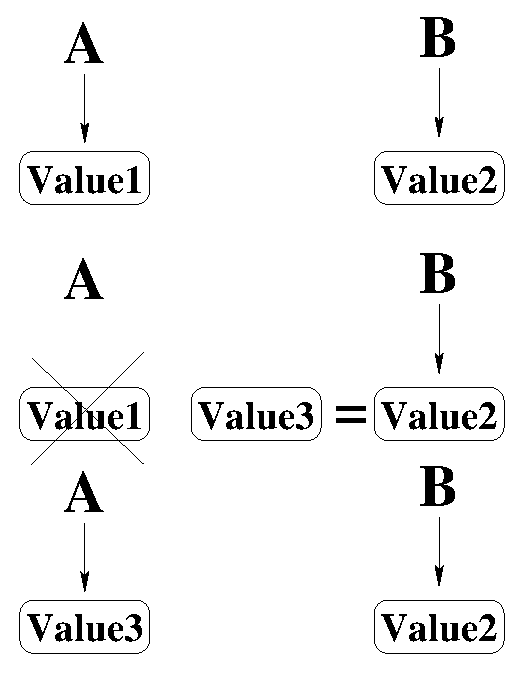
\includegraphics[scale=0.7]{value_semantic.eps}
\caption{The value semantic}
\end{center}
\end{figure}

\subsection{The reference semantic}
The memory management in the case of the reference semantic is very different. This time, each object is a pointer on a value and
different objects can share the same value. Then, you want to deallocate a given value only once all references on it were cleared.
For this purpose, you need to keep the count of the number of references currently used for each value. That's the meaning of the
field {\it Ref\_Counter} in the Any implementation.

When you create an Any, this field is set to 0. When you finalize an Any, the {\it Ref\_Counter}
is decreased and the value deallocate only if if it reaches 0. At last, in the case of an assignment, you just add one to {\it Ref\_Counter}
saying than one more reference on the value was created. Figure 6.2 on page \pageref{fig:refMemManag}
show you the assignment.
\begin{figure}
\label{fig:refMemManag}
\begin{center}
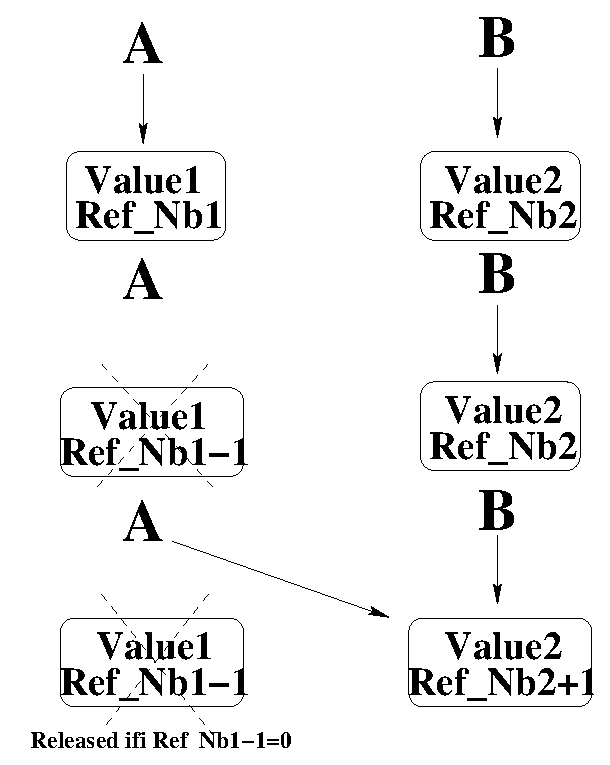
\includegraphics[scale=0.7]{reference_semantic.eps}
\caption{The reference semantic}
\end{center}
\end{figure}


\subsection{A controlled type}
\paragraph{}The easiest way to provide memory management for a given type in
 Ada is to derive from the Controlled object. This way, you have access
to every initialization, assignment and finalization of your objects. In the case of the Any type, the behavior of each of these
operations is dependant of the current semantic. That's why we put the field {\it As\_Reference} telling us what the current semantic is.
By default, this field is set to {\it False} by the Initialize method since it provides the behavior that the user is expected.
The only places where it is put to {\it True} are the creation of a request and the method {\it Add\_Item} of {\it CORBA.NVList}.
\paragraph{}To sum up all of it, here is the actual code for the Any type memory management (except I took off the lines concerning
thread-safe implementation). Note that the counter is used in the value
semantic too since the same value could be pointed by an Any with a value semantic and another one with a reference semantic.
\begin{verbatim}
   procedure Initialize (Object : in out Any) is
   begin
      Object.Ref_Counter := new Natural'(0);
   end Initialize;

   procedure Adjust (Object : in out Any) is
   begin
      if Object.As_Reference then
         Inc_Usage (Object);
      else
         if Get_Value (Object) /= Null_Content_Ptr then
            Object.The_Value := new Any_Content_Ptr'
               (Duplicate (Get_Value (Object)));
         else
            Object.The_Value := new Any_Content_Ptr'(Null_Content_Ptr);
         end if;
         Object.Ref_Counter := new Natural'(1);
      end if;
   end Adjust;

   procedure Finalize (Object : in out Any) is
   begin
      Dec_Usage (Object);
   end Finalize;

   procedure Inc_Usage (Obj : in Any) is
   begin
      Obj.Ref_Counter.all := Obj.Ref_Counter.all + 1;
   end Inc_Usage;

   procedure Dec_Usage (Obj : in out Any) is
   begin
      if Obj.Ref_Counter.all > 1 then
         Obj.Ref_Counter.all := Obj.Ref_Counter.all - 1;
      else
         if Obj.The_Value.all /= Null_Content_Ptr then
            Deallocate (Obj.The_Value.all);
         end if;
         Deallocate_Any_Content_Ptr (Obj.The_Value);
         Deallocate (Obj.Ref_Counter);
      end if;
   end Dec_Usage;
\end{verbatim}

%%% Thread-safe Anys
\section{Thread-safe Anys}
\paragraph{} The fact that some values are pointed to by several Any objects raises a problem in the case of a multi task environment.
In such a case, you'll have to make sure that two Anys are not using the same value at the same time or that one is not reading a value
that another in changing.
\paragraph{}In order to achieve this goal, you have to control every access to the {\it The\_Value} and {\it Ref\_Counter} field of the
Any type and place some lock on each of them. This is done by encapsulating all access to an Any inside 4 methods :
{\it Get\_Value}, {\it Set\_Value}, {\it Get\_Counter} and {\it Set\_Counter}. 
On the other side, the {\it Any\_Lock} field of each Any object provides a lock, shared by all Any pointing to the same value
and insuring you that only one of them will access the Any at the same time (actually, only one if it is writing and several if they
are reading).
\paragraph{}As an example of this thread-safe implementation, here is the code of the {\it Get\_Value} adn {\it Set\_Value} methods :
\begin{verbatim}
   procedure Set_Value (Obj : in out Any; The_Value : in Any_Content_Ptr) is
   begin
      Obj.Any_Lock.Lock_W;
      Obj.The_Value.all := The_Value;
      Obj.Any_Lock.Unlock_W;
   end Set_Value;

   function Get_Value_Ptr (Obj : Any) return Any_Content_Ptr_Ptr is
      Content : Any_Content_Ptr_Ptr;
   begin
      Obj.Any_Lock.Lock_R;
      Content := Obj.The_Value;
      Obj.Any_Lock.Unlock_R;
      return Content;
   end Get_Value_Ptr;
\end{verbatim}

%%% NamedValue, NVList
%%%%%%%%%%%%%%%%%%%%%%
\chapter{NamedValue, NVList}
\label{NV-NVList}
\paragraph{}The two types presented here : {\it NamedValue} and {\it NVList} are used in the dynamic
invocation process to describe arguments to
be passed to a function. {\it NamedValue} describes a single argument while {\it NVList} describes a list of them.

%%% NamedValue
\section{NamedValue}

Here is the Ada specification of the {\it NamedValue} type found in the {\it CORBA} package :
\begin{verbatim}
   type Flags is new CORBA.Unsigned_Long;
   ARG_IN :        constant Flags;
   ARG_OUT :       constant Flags;
   ARG_INOUT :     constant Flags;

   type NamedValue is record
      Name :      CORBA.Identifier;
      Argument :  CORBA.Any;
      Arg_Modes : CORBA.Flags;
   end record;
\end{verbatim}

\paragraph{}The fields are very clear :
\begin{itemize}
\item{\bf Name} is the name of the argument
\item{\bf Argument} is its value, given as an Any
\item{\bf Arg\_Modes} is the mode of the argument
\end{itemize}

%%% NVList
\section{NVList}
\label{NVList}
\paragraph{}The {\it NVList} type is a simple list of {\it NamedValue} except the CORBA specification prefered encapsulating it
in an object reference defined in the package {\it CORBA.NVList}.
\paragraph{}As usual, we'll describe the implementation of the type itself before describing the methods on this type .

\subsection{Ada specification}

Here is the specification of this package in Ada :
\begin{verbatim}
package CORBA.NVList is

   type Ref is new CORBA.AbstractBase.Ref with null record;

   procedure Add_Item (Self       :    Ref;
                       Item_Name  : in Identifier;
                       Item_Type  : in CORBA.TypeCode.Object;
                       Value      : in System.Address;
                       Len        : in Long;
                       Item_Flags : in Flags);

   procedure Add_Item (Self       :    Ref;
                       Item_Name  : in Identifier;
                       Item       : in CORBA.Any;
                       Item_Flags : in Flags);

   procedure Add_Item (Self : Ref;
                       Item : CORBA.NamedValue);

   procedure Free (Self : Ref);
   procedure Free_Memory (Self : Ref);

   function Get_Count (Self : Ref) return CORBA.Long;

end CORBA.NVList;
\end{verbatim}
\paragraph{}Next to these specification, there is a constructor for {\it NVList} provided in the {\it CORBA.ORB} package. Here is its specification :
\begin{verbatim}
   procedure Create_List (Count    : in     CORBA.Long;
                          New_List :    out CORBA.NVList.Ref);
\end{verbatim}

\subsection{implementation}
\label{NVListImpl}

\paragraph{}Since the specification imposes the encapsulation of the list of NamedValues in an object reference, we had to define
a new descendant of {\it CORBA.Impl.Object} containing this list (Maybe should we precise that the only field of a
{\it CORBA.AbstractBase.Ref} is a {\it CORBA.Impl.Object} ?). The list by itself is provided by the {\it Sequences.Unbounded} package.
Here are the corresponding definitions :
\begin{verbatim}
package CORBA.NVList is

   type Ref is new CORBA.AbstractBase.Ref with null record;

   type Object is new CORBA.Impl.Object with private;
   type Object_Ptr is access all Object;
   (...)

private
   package NV_Sequence is new Sequences.Unbounded (CORBA.NamedValue);

   type Object is new CORBA.Impl.Object with record
      List : NV_Sequence.Sequence := NV_Sequence.Null_Sequence;
   end record;
   (...)
end CORBA.NVList;
\end{verbatim}

\subsection{methods on type NVList}

Here is the meaning of each method :
\begin{itemize}
\item{\bf Add\_Item} There are three Add\_Item methods. They all does the same : adding an argument to Self.
This new argument can be described in three different forms : either you give it as a {\it NamedValue}, already encapsulated, or you
can give it as an {\it Identifier} (the name of the argument), an {\it Any} (the value of the argument) and a flag (the mode of the
argument). You can even avoid to build the {\it Any} value yourself by giving a {\it Typecode.Object}, a value and the length of the value.
However, this last method is not implemented at this time.
\item{\bf Free, Free\_Memory} : They are implemented but don't do anything. Actually the Object type is sort of controlled and
the memory deallocation is automatic. No need for the user to think at it.
\item{\bf Get\_Count} returns the number of arguments in the argument list.
\end{itemize}
\paragraph{}The constructor method don't need any comment except that the parameter count is useless.

\subsection{Added methods on NVList}

\paragraph{}There are four added methods on the NVList type. The first ones deal with marshalling and unmarshalling
of an NVList (it just marshalls or unmarshalls all elements of the list that should be marshalled or unmarshalled).
The two last are a constructor and a destructor for the Object type. Here are all the specifications :
\begin{verbatim}
   procedure Marshall (Buffer : access Broca.Buffers.Buffer_Type;
                       Data   : Ref);
   procedure Unmarshall (Buffer : access Broca.Buffers.Buffer_Type;
                         Data : in out Ref);

   function Create_Object return Object_Ptr;
   procedure Finalize (Obj : in out Object);
\end{verbatim}
\paragraph{}Just notice that {\it Create\_Object} creates an empty object, this means without any NVList associated and that the type
{\it CORBA.NVList.Ref} is controlled as a descendant of a controlled type.

%%% ExceptionList and ContextList
%%%%%%%%%%%%%%%%%%%%%%%%%%%%%%%%%
\chapter{ExceptionList, Contextlist}
\paragraph{}If you look for these two packages in the CORBA specification (v2.3),
I don't thing you'll find something interesting. They simply
do not exist. However they are needed by the dynamic invocation and thus, some issues were issued by the AdaBroker team
concerning this point. The packages presented here are a kind of translation of the C$^{++}$ Mapping specification, adapted to Ada.
We hope it will become part of the next specification of the Ada Mapping.
\paragraph{}Due to the similitudes between these packages and the NVList package, this chapter is not so precise than the others.
Please report to section section \ref{NVList} page \pageref{NVList} for further details.

%%% specification
\section{The Ada Specifications}
Here is the Ada specifications of these packages :
\begin{verbatim}
package CORBA.ExceptionList is

   type Ref is new CORBA.AbstractBase.Ref with null record;

   function Get_Count (Self : in Ref)
                       return CORBA.Unsigned_Long;
   procedure Add (Self : in Ref;
                  Exc : in CORBA.TypeCode.Object);
   function Item (Self : in Ref;
                  Index : in CORBA.Unsigned_Long)
                  return CORBA.TypeCode.Object;
   procedure Remove (Self : in Ref;
                     Index : in CORBA.Unsigned_Long);
end CORBA.ExceptionList;


package CORBA.ContextList is

   type Ref is new CORBA.AbstractBase.Ref with null record;

   function Get_Count (Self : in Ref)
                       return CORBA.Unsigned_Long;
   procedure Add (Self : in Ref;
                  Exc : in CORBA.String);
   function Item (Self : in Ref;
                  Index : in CORBA.Unsigned_Long)
                  return CORBA.String;
   procedure Remove (Self : in Ref;
                     Index : in CORBA.Unsigned_Long);
end CORBA.ContextList;
\end{verbatim}

\paragraph{}Next to these specification, there are two constructors for {\it ExceptionList} and {\it ContextList} provided in the package
{\it CORBA.ORB} :
\begin{verbatim}
   procedure Create_List (New_List : out CORBA.ExceptionList.Ref);
   procedure Create_List (New_List : out CORBA.ContextList.Ref);
\end{verbatim}

%%% Implementation
\section{Implementation}
\paragraph{}The implementation is mapped from {\it CORBA.NVList}. Thus we won't detail it here. Please report to section 
\ref{NVListImpl} on page \pageref{NVListImpl} and replace {\it NamedValue} by {\it TypeCode} for {\it ExceptionList}
or by {\it CORBA.String} for {\it ContextList}.

%%% Methods
\section{Methods}
\paragraph{}Here is a very brief description of each method of these packages :
\begin{itemize}
\item {\bf Get\_Count} : returns the number of element in the list
\item {\bf Add} : adds an element at the end of the list
\item {\bf Item} : returns the element at the given index in the list
\item {\bf Remove} : removes an element from the list
\end{itemize}
\paragraph{}The constructor methods don't need any comment.

%%% Added methods
\section{Added methods}
\paragraph{}There are first two methods added in both {\it ExceptionList} and {\it ContextList} :
\begin{itemize}
\item {\bf Create\_Object} : it is the constructor of the Object type. Only used by the constructor of the Ref type actually.
\item {\bf Finalize} : it is the destructor of the Object type. You can notice here that these type are controlled.
So the user don't have to take care of the memory he uses.
\end{itemize}
\paragraph{}The last method only exists in {\it ExceptionList} : {\bf Search\_Exception\_Id}. It is a searching function that returns the
index of the first {\it TypeCode} from the list denoting an exception called {\it Name}. That's useful in the {\it Invoke} method
of the package {\it CORBA.Request}.


%%% Request
%%%%%%%%%%%
\chapter{Request}

\paragraph{}The {\it Request} package is the heart of the dynamic invocation interface. It's the package that allows you to specify
a request, to invoke it and to get the result of it (if there is one). As usual now, we'll give the specification of this package before
detailing its implementation and the different methods provided. At last, we'll discuss the way the {\it Invoke} method deals with
exceptions.

%%% specification
\section{The Ada Specification}
\paragraph{} The Ada specification of the request package is the following :
\begin{verbatim}

package CORBA.Request is

   type Object is private;

   procedure Add_Arg
     (Self      : in out Object;
      Arg_Type  : in     CORBA.TypeCode.Object;
      Value     : in     System.Address;
      Len       : in     Long;
      Arg_Flags : in     Flags);

   procedure Add_Arg
     (Self : in out Object;
      Arg  : in     NamedValue);

   procedure Invoke
     (Self         : in out Object;
      Invoke_Flags : in     Flags  := 0);

   procedure Delete (Self : in out Object);

   procedure Send
     (Self         : in out Object;
      Invoke_Flags : in     Flags  := 0);

   procedure Get_Response
     (Self         : in out Object;
      Invoke_Flags : in     Flags  := 0);

   function Poll_Response (Self : in Object) return Boolean;

end CORBA.Request;
\end{verbatim}

\paragraph{}Next to this specification, there are two constructors for the type {\it CORBA.Request.Ref} provided in the {\it CORBA.Object}
package. Here is their Ada specification :
\begin{verbatim}
   procedure Create_Request
     (Self      : in     Ref;
      Ctx       : in     CORBA.Context.Ref;
      Operation : in     Identifier;
      Arg_List  : in     CORBA.NVList.Ref;
      Result    : in out NamedValue;
      Request   :    out CORBA.Request.Object;
      Req_Flags : in     Flags);

   procedure Create_Request
     (Self      : in     Ref;
      Ctx       : in     CORBA.Context.Ref;
      Operation : in     Identifier;
      Arg_List  : in     CORBA.NVList.Ref;
      Result    : in out NamedValue;
      Exc_List  : in     ExceptionList.Ref;
      Ctxt_List : in     ContextList.Ref;
      Request   :    out CORBA.Request.Object;
      Req_Flags : in     Flags);
\end{verbatim}
\paragraph{}Actually, if you look in the current Ada mapping, you'll only find the first constructor. The second one is not provided
but was issued as an issue to the OMG by the Adabroker team. Maybe the next CORBA specification will include it.

%%% Implementation
\section{Implementation}
\paragraph{}Since the Request package is the heart of the dynamic invocation mechanism, you find in its implementation all the components
needed to realise an invocation. Here is the definition of the {\it Request.Object} type :
\begin{verbatim}
   type Object is
      record
         Ctx        : CORBA.Context.Ref;
         Target     : CORBA.AbstractBase.Ref;
         Operation  : CORBA.Identifier;
         Args_List  : CORBA.NVList.Ref;
         Result     : CORBA.NamedValue;
         Exc_List   : CORBA.ExceptionList.Ref;
         Ctxt_List  : CORBA.ContextList.Ref;
         Req_Flags  : CORBA.Flags;
      end record;
\end{verbatim}
\paragraph{}Most of the fields are understandable but let's detail a little bit each of them :
\begin{itemize}
\item {\bf Ctx} : the context of the invocation. The context object is not described in this documentation since this functionnality is not
currently available in AdaBroker. However, the {\it CORBA.Context} package exists and its constant {\it Nil\_Ref} can be used.
\item {\bf Target} : the object on which the invocation will be done.
\item {\bf Operation} : the operation to be invoked.
\item {\bf Args\_List} : the list of arguments to pass to this operation. You can put a null list here at the creation of a request
and add some arguments to the request later if you want (by using {\it Add\_Arg}).
\item {\bf Result} : the type of the result to be returned. You may say it should be a {\it TypeCode} since it only carries a type. The fact
is that the result will be put there after computation. So you must give an {\it Any} but it can have no value.
\item {\bf Exc\_List} : the list of the exception potentially raised by the method to be invoked, given as a list of {\it TypeCode}.
\item {\bf Ctxt\_List} : the list of the context elements to be passed to the invoked method. This field is not used for the moment.
\item {\bf Req\_Flags} : some flags dealing with the memory management. Not used for the moment.
\end{itemize}


%%% Methods
\section{Methods on Request Objects}
\paragraph{}Here is the description of all methods of the {\it CORBA.Request} object and of the constructors of this type. I must precise
here that only the blocking invocation is provided by AdaBroker at this moment which means that the methods {\it Send}, {\it Get\_Response},
and {\it Poll\_Response} are not implemented. Note also that the different arguments dealing with contexts are not managed since contexts
are not implemented.

\begin{itemize}
\item{\bf Create\_Request} These methods take as parameters all what is needed to create a request object. The first one just forgets
the exception and context lists and uses default values. Each argument of these functions is directly put into the
coresponding field of the created request object.

\item{\bf Add\_Arg} These methods allows you to add an argument to a request. You can either give directly a NamedValue that encapsulates 
all the fields of an argument or give each of these fields. Here is their meaning :
\begin{itemize}
\item{\it Arg\_type} is the type of the argument given as a TypeCode.
\item{\it Value} is the value of the argument. Together with the argument type, you have an Any value : a value and its description.
\item{\it Len} is the length of the argument. It is actually not used.
\item{\it Arg\_Flags} is a flag describing the mode of the argument.
 There is only three possible values : {\it CORBA.ARG\_IN}, {\it CORBA.ARG\_INOUT} and {\it CORBA.ARG\_OUT}.
\end{itemize}

\item{\bf Invoke} This is the key method for a regular invocation. It takes a request and makes the invocation. What it does is
marshalling the request first (object reference, operation name, arguments and perhaps context), then calling the ORB to send the
buffer to the server and at last waiting for the response. When the reply comes, it unmarshalls the result (or the exception if any)
and puts it in the {\it Result} field (or raise it). Note that the call is blocking : {\it Invoke} will only return once the result is known.

\item{\bf Delete} deletes a request and frees the associated memory.

\item{\bf Send} This method is the pending of {\it Invoke} for non blocking calls. It only marshalls the elements of the request and calls
the ORB but does not wait for any answer. It means that it gives you the control right back without waiting the processing of your
call to finish.

\item{\bf Get\_Response} This is the complement of the {\it Send} method. It allows you to get the result of an invocation made with 
{\it Send}. This method is blocking if the result is not yet ready.

\item{\bf Poll\_Response} This allows you to know if a given result is ready or not. This way, you are able 
call {\it Get\_Response} only when you know you won't wait.
\end{itemize}

%%% Exceptions
\section{Dealing with exceptions}
\paragraph{}As in the static case, an invocation can result in raising an exception. This one should be raised in the client by the
{\it Invoke} method as it was raised by the dedicated proxy in the static case (see end of subsection \ref{StaticExcp} on page
\pageref{StaticExcp}).
\paragraph{}The problem you're faced with, in the dynamic case is that the exception to be raised is not defined since you don't use
the generated files. The solution was to raise a dedicated exception : {\it UnknownUserException}. Here is its definition in the
{\it CORBA} package :
\begin{verbatim}
   UnknownUserException : exception;
   type UnknownUserException_Members is
     new CORBA.IDL_Exception_Members with record
        IDL_Exception : Any;
     end record;

   procedure Get_Members
     (From : Ada.Exceptions.Exception_Occurrence;
      To   : out UnknownUserException_Members);
\end{verbatim}
\paragraph{}This exception contains an Any in its member, which allows us to put any member in it. This way, in case of exception,
the {\it Invoke} method just has to unmarshall the member in an Any and raise an {\it UnknownUserException}. In order to make it
clear, here is a part of the code of the {\it Invoke} method :
\begin{verbatim}
    case Send_Request_Result is
       (...)
       when Broca.GIOP.Sr_User_Exception =>
          declare
             Exception_Repo_Id : CORBA.RepositoryId
               := Broca.CDR.Unmarshall (Handler.Buffer'Access);
             Index : CORBA.Unsigned_Long
               := CORBA.ExceptionList.Search_Exception_Id
               (Self.Exc_List, Exception_Repo_Id);
          begin
             if Index > 0 then
                declare
                   Member : UnknownUserException_Members;
                begin
                   Member.IDL_Exception := CORBA.Get_Empty_Any
                     (CORBA.ExceptionList.Item (Self.Exc_List,
                                                Index));
                   Broca.CDR.Unmarshall_To_Any
                     (Handler.Buffer'Access,
                      Member.IDL_Exception);
                   Broca.GIOP.Release (Handler);
                   Broca.Exceptions.User_Raise_Exception
                     (UnknownUserException'Identity,
                      Member);
                end;
             else
                Broca.GIOP.Release (Handler);
                raise Program_Error;
             end if;
          end;
\end{verbatim}
\paragraph{}I will just add here that this mechanism and the {\it UnknownUserException} are not provided by the CORBA specification
but are present in the C$^{++}$ Mapping.
We thus copied it in Ada and proposed it as a revision of the specification to the OMG.


%%% Marshall
%%%%%%%%%%%%
\chapter{Marshall, Unmarshall}

\paragraph{}This chapter does not deal with a specific package provided by the CORBA specification but with the way {\it TypeCode}s and
{\it Any}s are marshalled and unmarshalled. Note that most of the marshall and unmarshall operations are provided in the
{\it Broca.Cdr} package, so this chapter could be named Broca.Cdr and deal with a package...
\paragraph{}There is actually no big deal in marshalling {\it Any}s and {\it TypeCode}s but there's some useful things to know about it.
I'll first describe the way the marshalling/unmarshalling is implemented before giving some details of the GIOP protocol.

%%% Implementation
\section{Implementation}
\paragraph{}As for any defined type in CORBA, there is simply a {\it Marshall} and an {\it Unmarsdhall} method for both the {\it Any}
and the {\it TypeCode} type. The methods for {\it TypeCode} are very simple : depending of the kind of TypeCode they (un)marshall
the different fields to (un)marshall.

\paragraph{} For the Any, it is something different and two more
methods are defined : {\it Marshall\_From\_\-Any} and {\it Unmarshall\_To\_Any}. They are called respectively by {\it Marshall} and
{\it Unmarshall} and are able to marshall or unmarshall the value field of an Any according to the GIOP protocol.

%%% GIOP
\section{GIOP}
\paragraph{}The only thing interesting then is to know which fields are marshalled for each kind of value and in which order.
This is given in chapter 15 of \cite{OMG} but here it is again. Each parameter is
written in the form {\it type (name)} where {\it type} describes the parameter type and {\it name} the parameter meaning. 
Some parameters are repeated in sequence. It is written in the form {\it \{parameters\}}.

\begin{center}
\begin{small}
\begin{tabular}{|l|p{10cm}|}
\hline
{\it TC\_Kind} &
{\it Any}s in {\it Parameter} \\ \hline \hline
 {\bf Tk\_Null} &
-none-\\ \hline
{\bf Tk\_Void} &
-none-\\  \hline
{\bf Tk\_Short} &
-none-\\  \hline
{\bf Tk\_Long} &
-none-\\  \hline
{\bf Tk\_Ushort} &
-none-\\  \hline
{\bf Tk\_Ulong} &
-none-\\  \hline
{\bf Tk\_Float,} &
-none-\\  \hline
\end{tabular}
\end{small}
\end{center}
\begin{center}
\begin{small}
\begin{tabular}{|l|p{10cm}|}
\hline
{\it TC\_Kind} &
{\it Any}s in {\it Parameter} \\ \hline \hline
{\bf Tk\_Double} &
-none-\\  \hline
{\bf Tk\_Boolean} &
-none-\\  \hline
{\bf Tk\_Char} &
-none-\\  \hline
{\bf Tk\_Octet} &
-none-\\  \hline
{\bf Tk\_Any} &
-none-\\  \hline
{\bf Tk\_TypeCode} &
-none-\\  \hline
{\bf Tk\_Principal} &
-none-\\  \hline
{\bf Tk\_Objref} &
string (RepositoryId),

string (Name)\\  \hline
{\bf Tk\_Struct} &
string (RepositoryId),

string (Name),

ulong (count)

\{string (member name),

TypeCode (member type)\}\\  \hline
{\bf Tk\_Union} &
string (RepositoryId),

string (Name),

TypeCode (discriminator type),

long (default used),

ulong (count)

\{{\it discriminator type}\footnotemark[1]
(label value),

string (member name),

TypeCode (member type)\}\\  \hline
{\bf Tk\_Enum} &
string (RepositoryId),

string (Name),

ulong (count)

\{string (member name)\}\\  \hline
{\bf Tk\_String} &
ulong (max length\footnotemark[2])\\  \hline
{\bf Tk\_Sequence} &
TypeCode (element type),

ulong (max length\footnote[3])\\  \hline
{\bf Tk\_Array} &
TypeCode (element type),

ulong (length)\\  \hline
{\bf Tk\_Alias} &
string (RepositoryId),

string (Name),

TypeCode (aliased type)\\  \hline
{\bf Tk\_Except} &
string (RepositoryId),

string (Name),

ulong (count)

\{string (member name),

TypeCode (member type)\}\\  \hline
{\bf Tk\_Longlong} &
-none-\\  \hline
{\bf Tk\_Ulonglong} &
-none-\\  \hline
{\bf Tk\_Longdouble} &
-none-\\  \hline
{\bf Tk\_Widechar} &
-none-\\  \hline
{\bf Tk\_Wstring} &
ulong (max length\footnotemark[4])\\  \hline
\end{tabular}
\end{small}
\end{center}
\footnotetext[1]{The type of union label values is determined by the second parameter, {\it discriminator type}}
\footnotetext[2]{for unbounded strings, this value is 0.}
\footnotetext[3]{for unbounded sequences, this value is 0.}
\footnotetext[4]{for unbounded wide strings, this value is 0.}
\begin{center}
\begin{small}
\begin{tabular}{|l|p{10cm}|}
\hline
{\it TC\_Kind} &
{\it Any}s in {\it Parameter} \\ \hline \hline
{\bf Tk\_Fixed} &
ushort (digits),

short (scale)
\\  \hline
{\bf Tk\_Value} &
string (RepositoryId),

string (Name, may be empty),

short (ValueModifier),

TypeCode (Concrete Base)\footnotemark[5],

ulong (count)

\{string (member name),

TypeCode (member type)

short (Visibility)\}\\  \hline
{\bf Tk\_Valuebox} &
string (RepositoryId),

string (Name),

TypeCode (type)\\  \hline
{\bf Tk\_Native} &
string (RepositoryId),

string (Name)\\  \hline
{\bf Tk\_Abstract\_Interface} &
string (RepositoryId),

string (Name)\\  \hline
\end{tabular}
\end{small}
\end{center}
\footnotetext[5]{should be {\it Tk\_Null} if there is no concrete base}

\begin{thebibliography}{99}
\bibitem[OMG]{OMG} The Common Object Request Broker : Architecture and Specification \\ Revised Edition : June 1999
\bibitem[AdaM]{AdaMapping} Ada Language Mapping Specification - version 1.2 : May 2000
\end{thebibliography}

\end{document}
